\chapter*{Vorwort}

\textit{Dies ist das offizielle ToM+-Benutzerhandbuch, das von mir (Fabio Java) in englischer Sprache handschriftlich verfasst wurde, ohne Einsatz
irgendeines KI-Tools – weder in diesem Handbuch noch im Code, auf dem ToM+ basiert. Andere Sprachen
als Englisch wurden automatisch mit} \href{https://www.deepl.com/en/translator}
    {DeepL} übersetzt.\\

\textit{In einer Zeit der automatisierten Inhaltserstellung hebt sich dieses Handbuch von anderen ab, und Sie können
sicher sein, dass alle bereitgestellten Funktionen und die Benutzeroberfläche von Menschen verfasst wurden.
Das macht dieses Projekt unter allen Alternativen einzigartig: Genau zu wissen,
was der Code tut, ist der Schlüssel dazu, bewusst neue Funktionen zu entwickeln, Fehler zu beheben und
bei Bedarf anderen ToM+-Besitzern Unterstützung zu garantieren.}\\

\textit{ToM+ entwickelt sich dank seiner großen Community, die aus dem}
\href{https://www.twizy-forum.de/twiz-o-meter}
    {deutschen Twizy-Forum} hervorgegangen ist, ständig weiter. \textit{Wenn Sie 
ein ToM+-Gerät erwerben möchten, senden Sie mir bitte eine E-Mail an} \textbf{info.twizometer@gmail.com}.
\textit{Wenn Sie eine neue Funktion vorschlagen, einen Fehler oder sogar einen Tippfehler in diesem
Handbuch melden möchten, senden Sie mir bitte eine E-Mail oder erstellen Sie einen Pull-Request auf} \href{https://codeberg.org/fabio-java/ToM-Wizard}
    {Codeberg}.\\

\textit{Wenn Sie ein Standard-ToM oder ein BigToM besitzen, können Sie ebenfalls auf dieses Benutzerhandbuch zurückgreifen,
da die Funktionen im Wesentlichen identisch sind – mit Ausnahme des Standard-ToM, bei dem die Dashboard-Seite
und die 3D-Ladeseiten fehlen.}\\

\textit{ToM ist kein kommerzielles Produkt und wird von einem Hobbybastler wie mir in Handarbeit hergestellt; jedes 
Exemplar ist ein Unikat und muss als Prototyp betrachtet werden, ohne CE-Zeichen oder sonstige 
offizielle Prüfungen. Das Twiz O’meter liest Daten vom CAN-Bus aus, ohne dass
Änderungen am Fahrzeug vorgenommen werden müssen; ich übernehme jedoch keine Haftung für dessen Einbau
und Nutzung.}\\

\textit{Diese Bedienungsanleitung wurde am 03.09.2026 auf die ESP-Firmware-Version 2.4 aktualisiert.}


\chapter{Beschreibung und Funktionsübersicht}

\section{Die wichtigsten Funktionen des ToM+}

ToM+ verfügt über zahlreiche Funktionen und kann im Zuge der Firmware-Entwicklung
laufend aktualisiert werden. In den folgenden Abschnitten werde ich Ihnen eine kurze Einführung in die
Funktionen geben, um Ihnen einen Eindruck von der Art des Produkts zu vermitteln, das ich später in dieser Anleitung näher erläutern werde.

\subsection{Ein neues Twizy-Armaturenbrett}

Da das Armaturenbrett unseres Twizy lediglich einige Werte wie die Geschwindigkeit und die
verbleibende Reichweite in Kilometern anzeigt, habe ich mich entschlossen, dieses coole Display zu entwickeln, das weitaus
mehr Daten anzeigt, indem es diese direkt vom CAN-Bus des Twizy über den OBD-Anschluss
im linken Handschuhfach ausliest. ToM „erfasst“ lediglich die vom Twizy gesendeten Werte und
zeigt sie dann auf dem LCD-Display an, was zahlreiche weitere Funktionen ermöglicht. ToM verfügt über einen winzigen,
aber leistungsstarken Speicher, der einige dieser Werte während der Fahrt speichern kann, um
Ihnen einen Fahrverlauf anzuzeigen. Dank dieser Speicherfunktion ist es möglich,
Ihre Konfigurationen und individuellen Einstellungen auf dem ToM zu speichern – selbst nach einem Firmware-Update.

\begin{figure}[H]
    \centering
    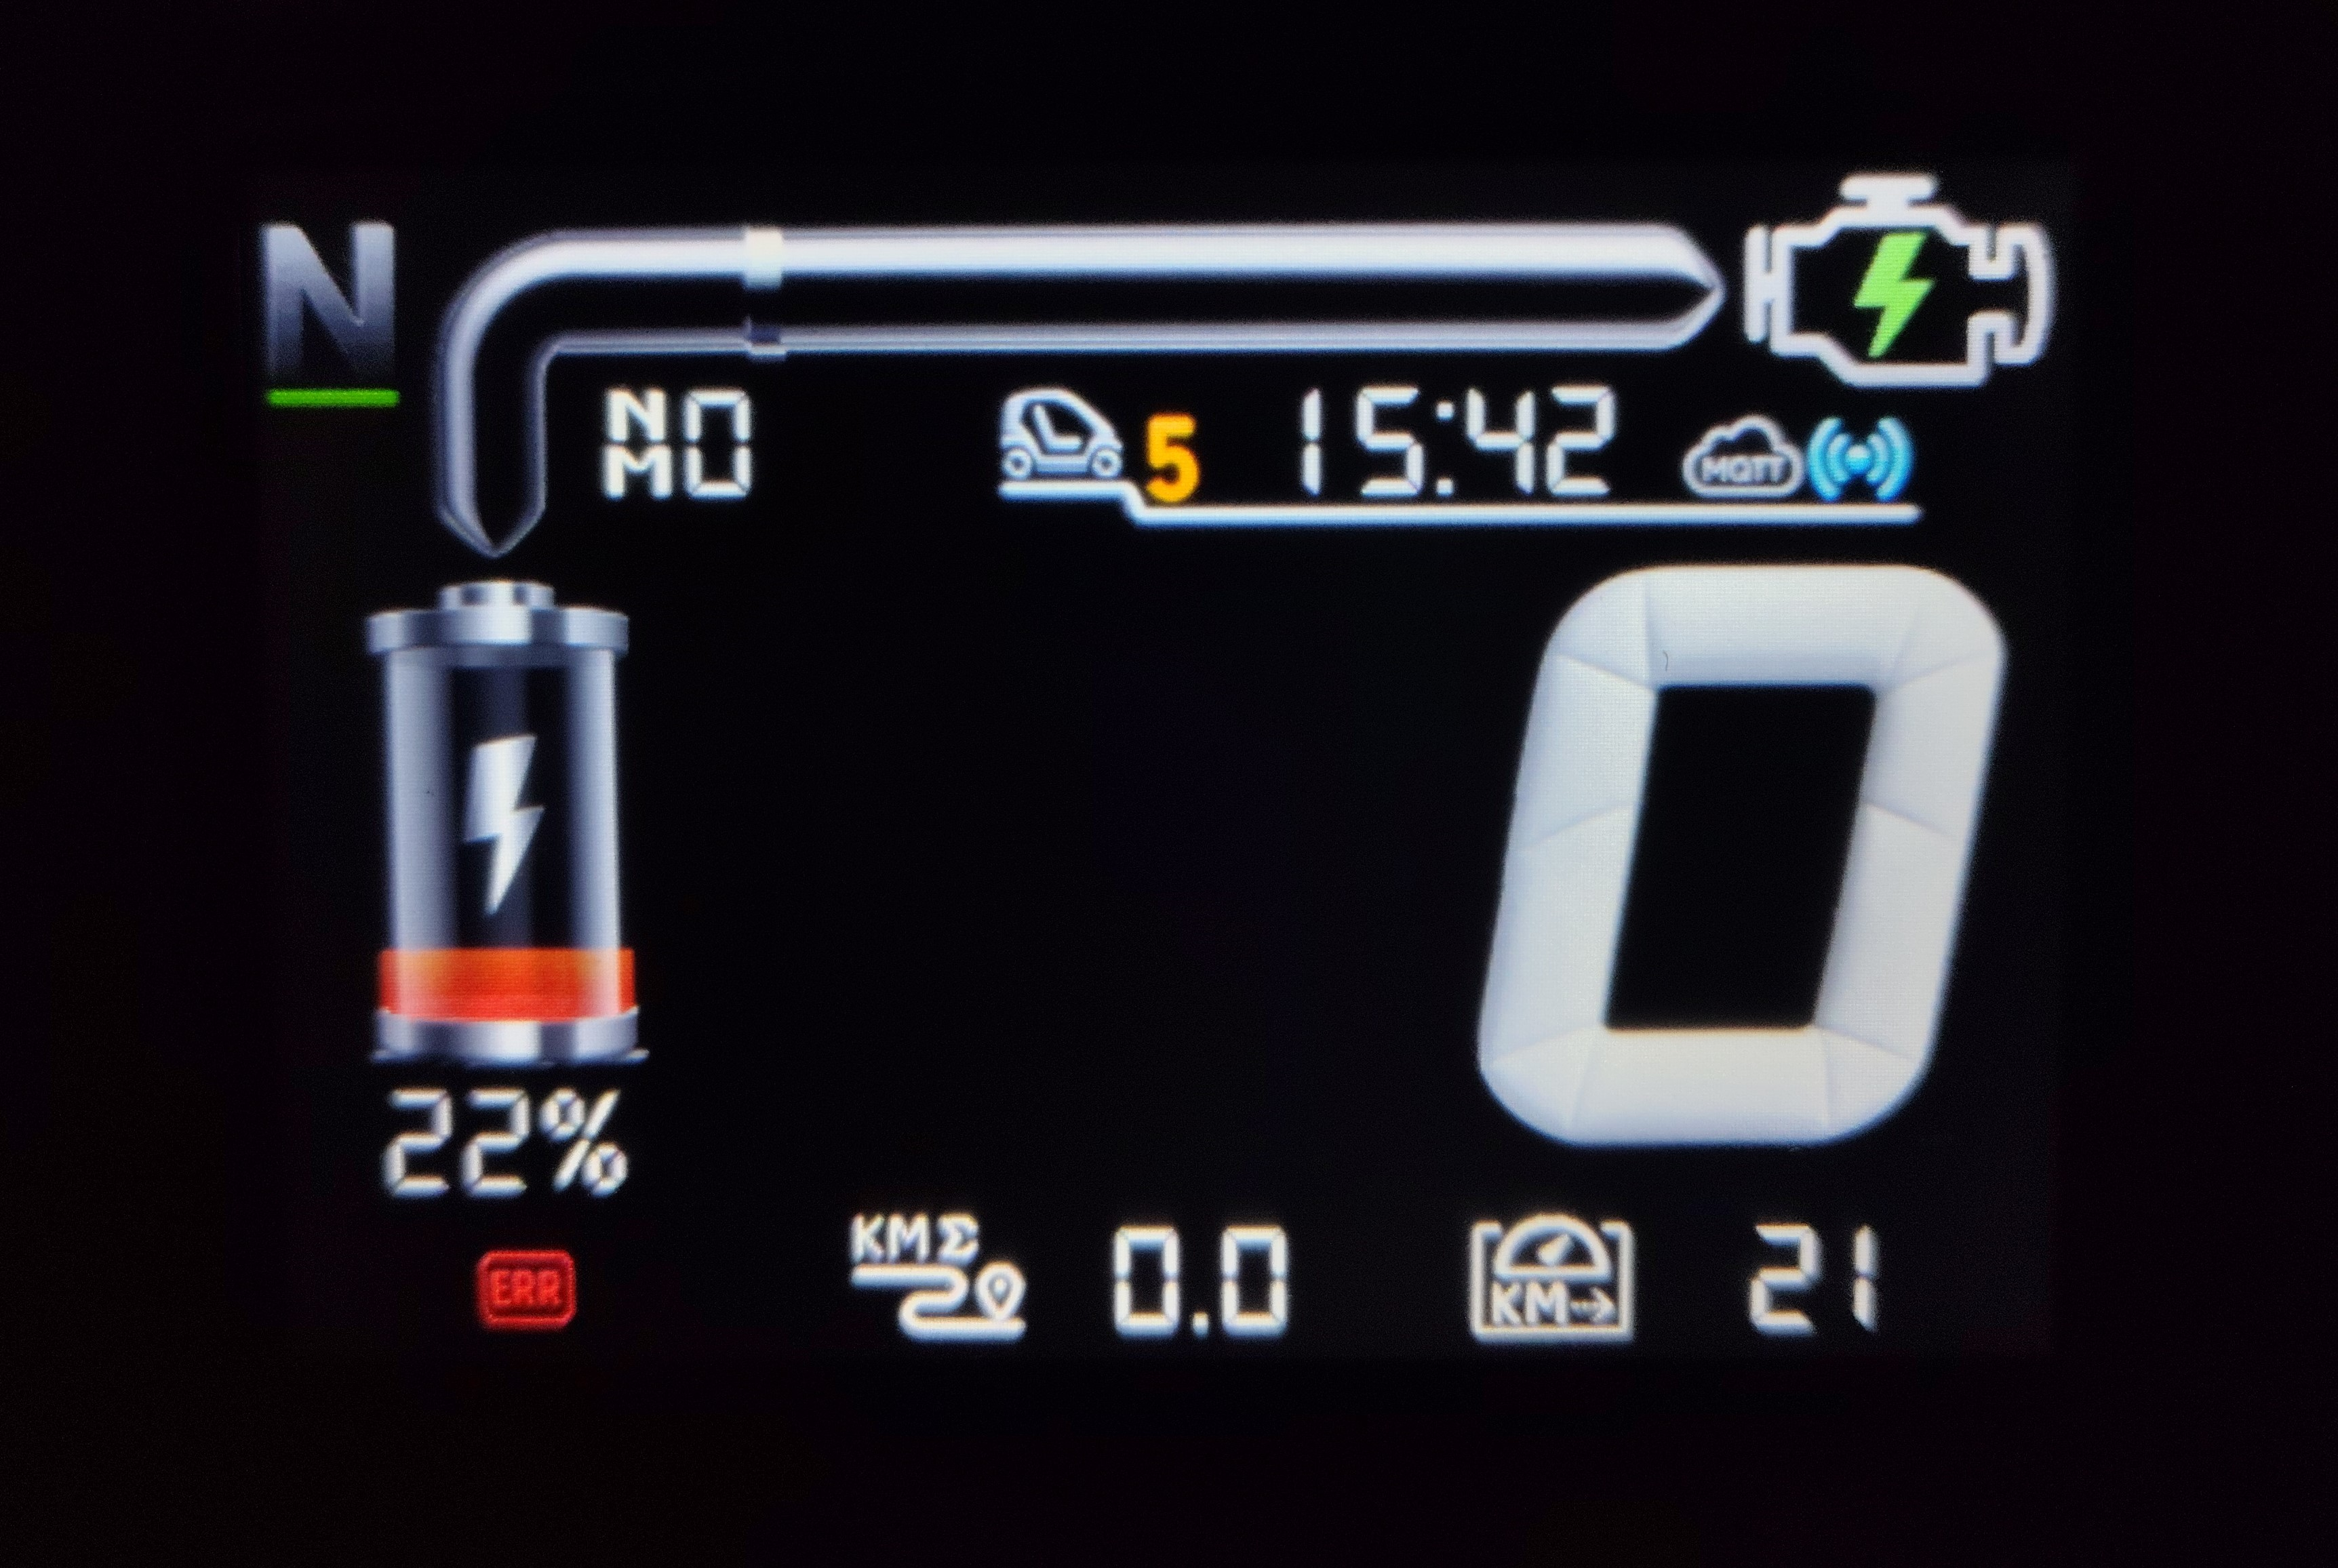
\includegraphics[width=0.8\textwidth]{figures/dashboard.jpg}
    \caption{Armaturenbrett des ToM+}
\end{figure}

Es versucht, den Stil des ursprünglichen Twizy-Armaturenbretts beizubehalten, jedoch mit einem moderneren und
3D-ähnlichen Erscheinungsbild.
Wie beim Original werden die Batterie, der Gang, die verbleibende Reichweite in Kilometern, die Geschwindigkeit und die Uhrzeit angezeigt.
Ich habe jedoch den genauen \textbf{Batterieprozentsatz}, das Motordrehmoment, einige Statussymbole, Fahrteninformationen und viele weitere Elemente hinzugefügt, die Sie nach Belieben konfigurieren können und auf die wir später noch im Detail eingehen werden.

Die Hauptseite ist anpassbar, und Sie können auswählen, was darauf angezeigt werden soll – ebenso wie auf den anderen Seiten, durch die Sie mithilfe der Taste blättern können, die Sie am Scheibenwischerhebel anbringen können.
Das allgemeine Erscheinungsbild der anderen Seiten ist in der Abbildung dargestellt, wobei ein Wert im Vordergrund und die anderen auf der linken Seite zu sehen sind. Im unteren Bereich
können Sie die angezeigte Seite ändern, indem Sie auf das entsprechende Symbol tippen.

\begin{figure}[H]
    \centering
    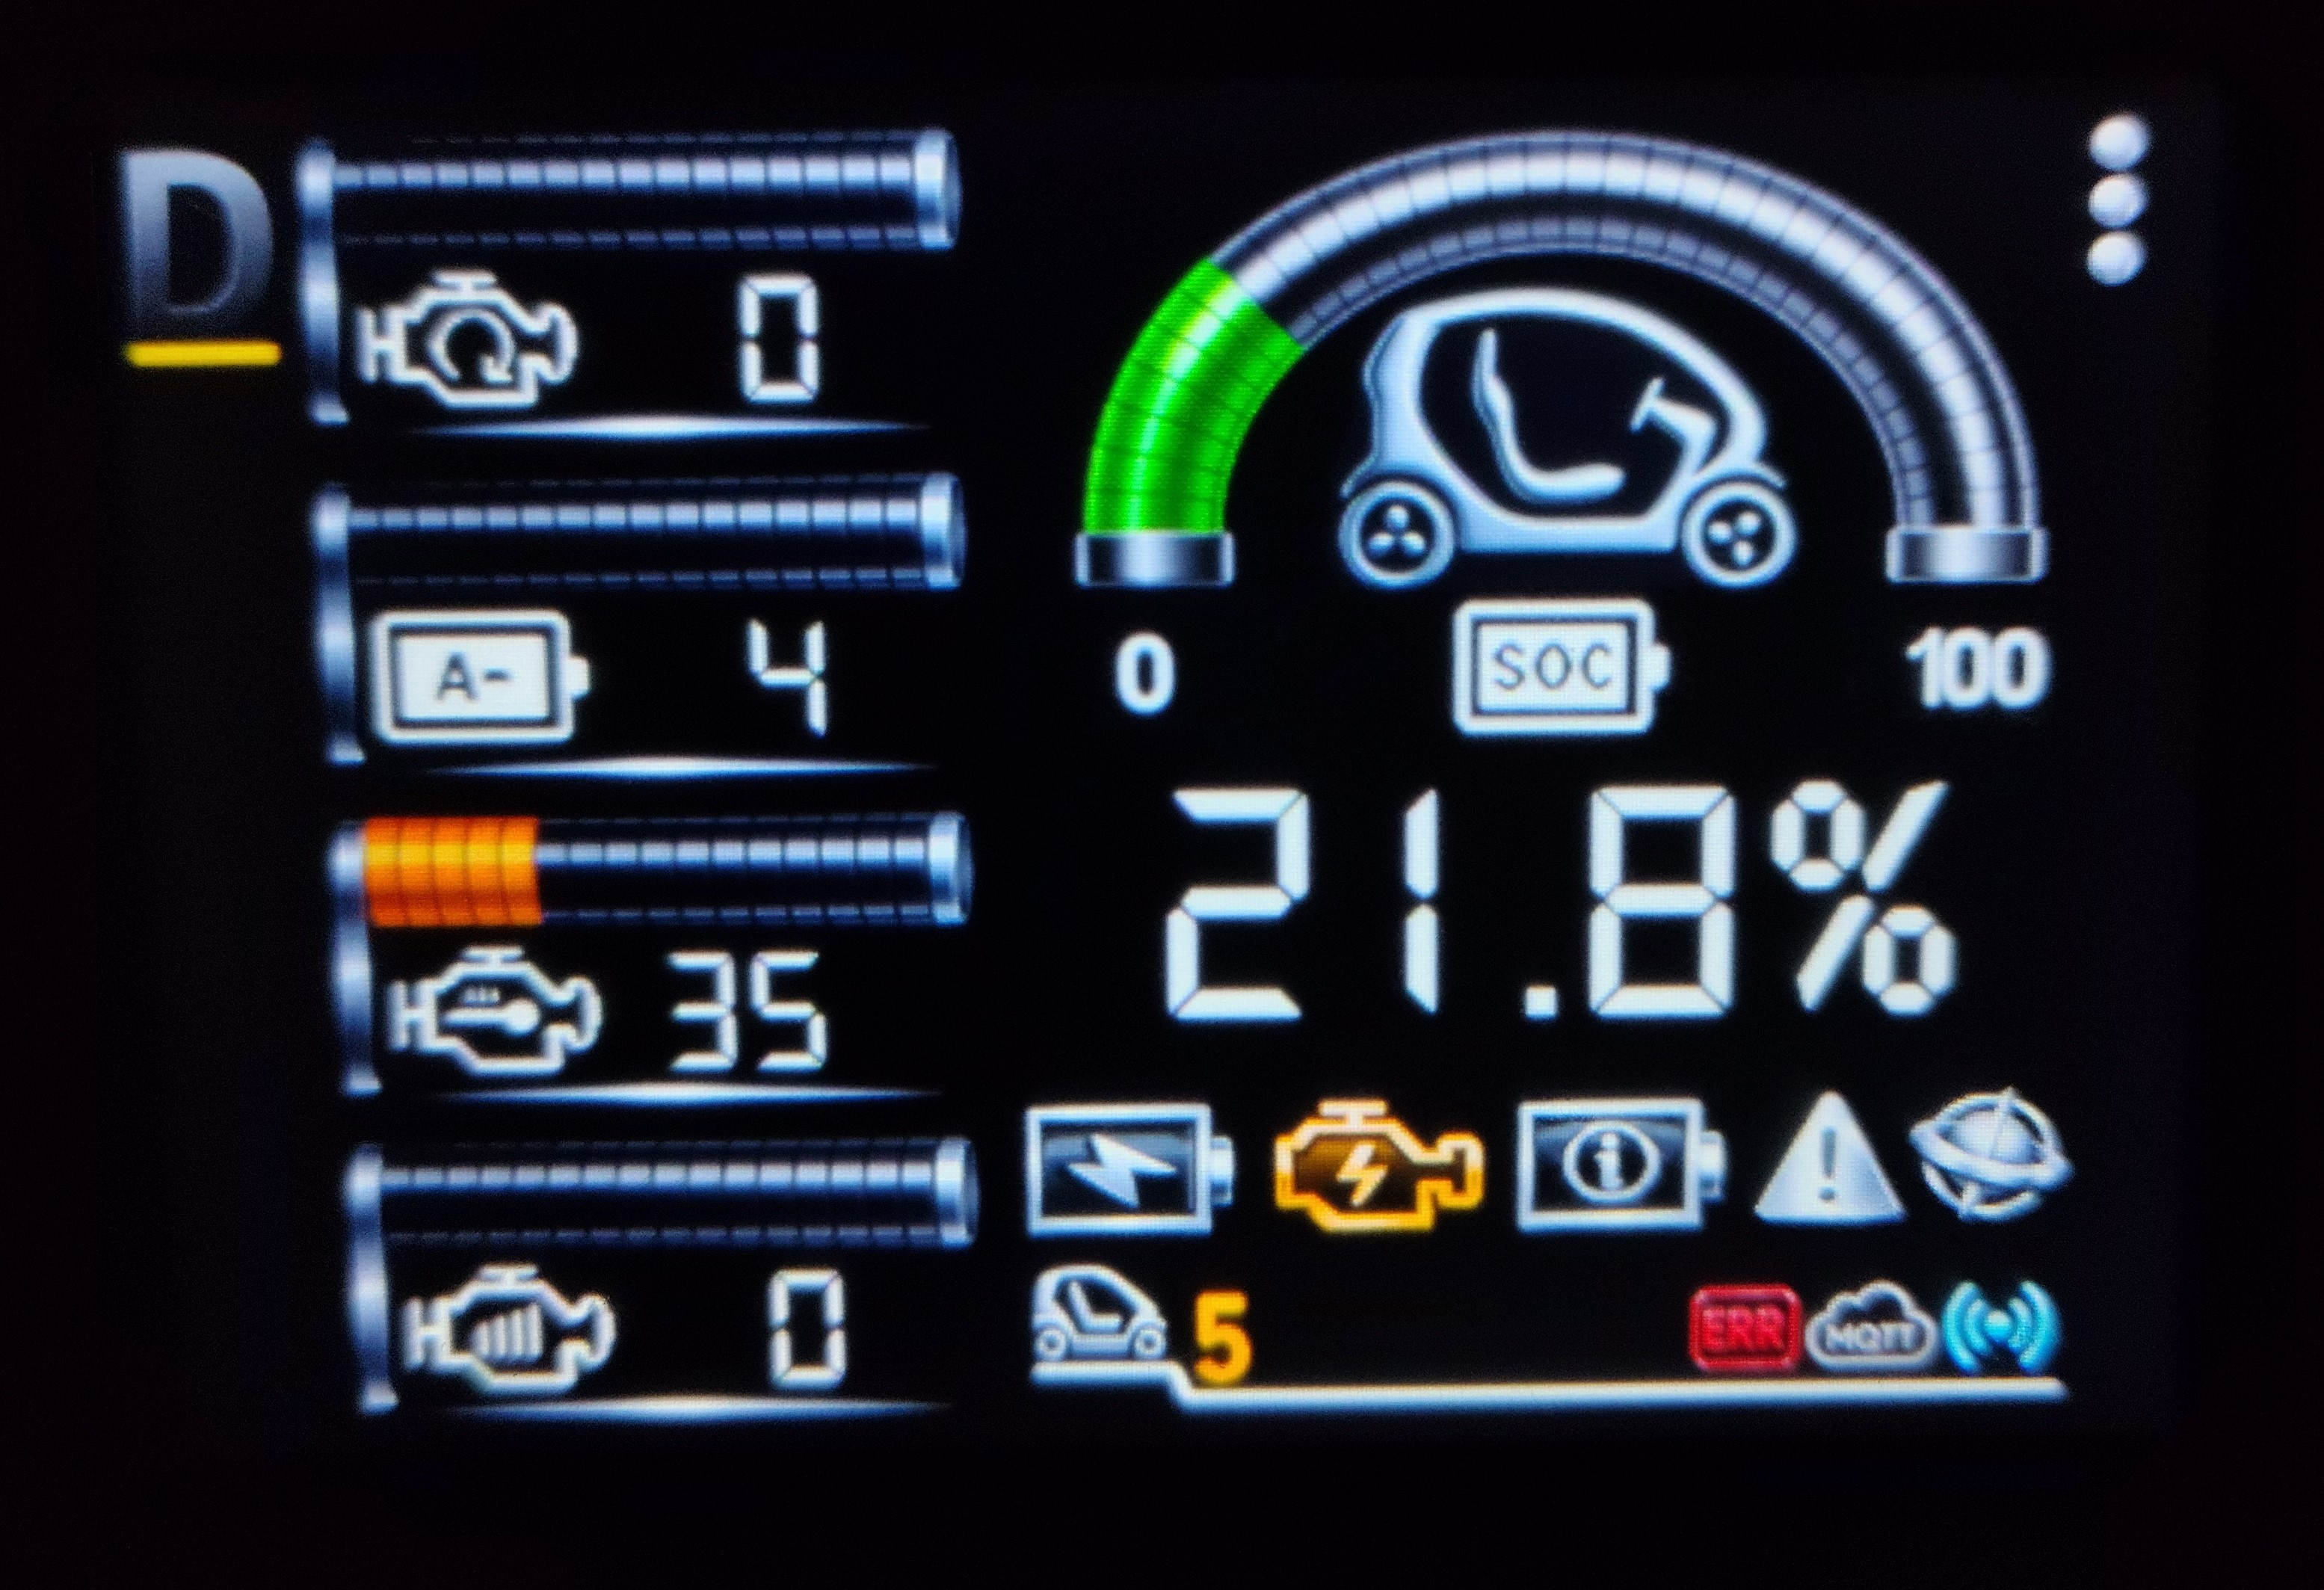
\includegraphics[width=0.8\textwidth]{figures/engine_page.jpg}
    \caption{Motorseite des ToM+}
\end{figure}

\subsection{WLAN-Verbindung}

Das in der schwarzen Box enthaltene ESP32-Board verfügt über die Fähigkeit, eine Verbindung zu einem WLAN-
Netzwerkzugangspunkt herzustellen. Sobald ToM+ verbunden ist, stehen Ihnen zahlreiche Möglichkeiten offen. So
kann dieses Gerät beispielsweise dazu verwendet werden, Daten von Ihrem Twizy an Ihren persönlichen \textbf{MQTT}
Broker übertragen, wo Sie diese Werte nutzen können, um Ihr Auto in Ihr IoT-System für die Hausautomation einzubinden. 

Dies ist nicht die einzige Funktion im Zusammenhang mit der WLAN-Fähigkeit, über die das ToM+ verfügt. Es kann 
auch als Zugangspunkt mit eigener SSID und eigenem Passwort fungieren und so ein privates Netzwerk ohne 
Internetverbindung erstellen. Auf diese Weise können Sie eine sichere Verbindung herstellen und \textbf{akzeptieren, das Verbindungsprofil}
aktiv zu halten, auch wenn keine Internetverbindung besteht (dies wird in der Regel 10 Sekunden nach der ersten Verbindung mit einer
Benachrichtigung auf Android-Smartphones angezeigt), und anschließend Ihre
weiteren Konfigurationen auf einigen Webseitenseiten vornehmen, die von ToM+ selbst gehostet werden. Geben Sie einfach
in Ihrem bevorzugten Browser die statische private IPv4-Adresse von ToM (\textbf{\textit{192.188.1.188}}) ein und genießen Sie es!

\begin{figure}[H]
    \centering
    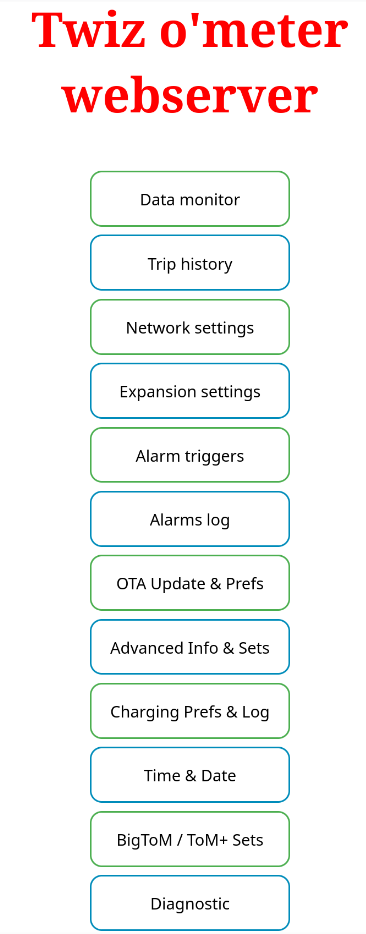
\includegraphics[
        width=\textwidth,
        height=0.75\textheight,
        keepaspectratio
    ]{figures/landing_page.png}
    
    \caption{Startseite des Webservers}
\end{figure}

Wie Sie in dieser neuen Version von ToM sehen können, ist der Webserver wesentlich umfassender und benutzerfreundlicher geworden. Sie können problemlos durch die Seiten navigieren und Ihr Gerät nach Ihren Wünschen konfigurieren. Der Webserver ist zudem responsiv, sodass Sie ihn auch auf Ihrem Smartphone oder Tablet nutzen können.

\subsection{ToM-Smartphone-App}

Neben den Firmware-Updates für das LCD und die Blackbox wird auch eine minimalistische Android-App
ständig auf dem neuesten Stand gehalten, mit der Sie die Echtzeitdaten Ihres Twizy über
Ihr Smartphone überwachen können. 

Das Layout versucht, die ursprüngliche grafische Benutzeroberfläche von ToM nachzubilden, und nutzt das \textbf{MQTT}-Protokoll, um
Werte von ToM+ an die App weiterzugeben und zu übertragen; daher müssen Sie die Konfiguration sowohl
in der App als auch auf der ToM+-MQTT-Seite vornehmen und dabei die IN- und OUT-Themen vertauschen. Die App wird
als \textbf{APK}-Datei bereitgestellt, ein gepacktes Installationsprogramm für Android-Anwendungen, mit dem
Sie diese App auch ohne Internetverbindung installieren können. Sie ist \href{https://www.mediafire.com/file/du7px1bzq0zzdxu/TwizOMeter_v3.1.2.apk/file}
    {hier klicken} verfügbar.

Möglicherweise müssen Sie in den Einstellungen Ihres Smartphones die Option „Apps aus unbekannten Quellen installieren“ aktivieren, um eine Datei
mit der Endung \textit{(.apk)} zu öffnen. Beim ersten Start wird möglicherweise ein Popup-Fenster angezeigt, in dem darauf hingewiesen wird, dass diese Anwendung
für eine ältere Android-Version entwickelt wurde, falls Sie ein neueres Smartphone besitzen: Klicken Sie einfach auf „OK“
und ignorieren Sie die Meldung (die App funktioniert einwandfrei). Hier sehen Sie eine Vorschau auf die Lade- und Einstellungsseite der App:

\begin{figure}[H]
    \centering
    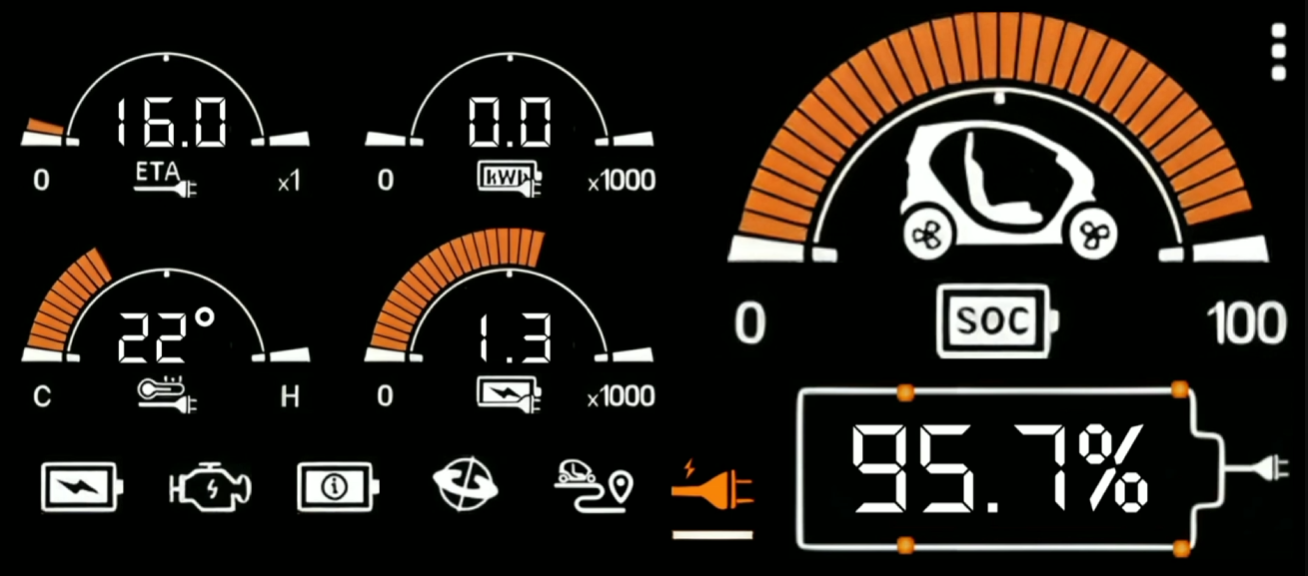
\includegraphics[width=0.8\textwidth]{figures/tom_app_charging.png}
    \caption{Ladeseite der ToM+-Android-App}
\end{figure}

\begin{figure}[H]
    \centering
    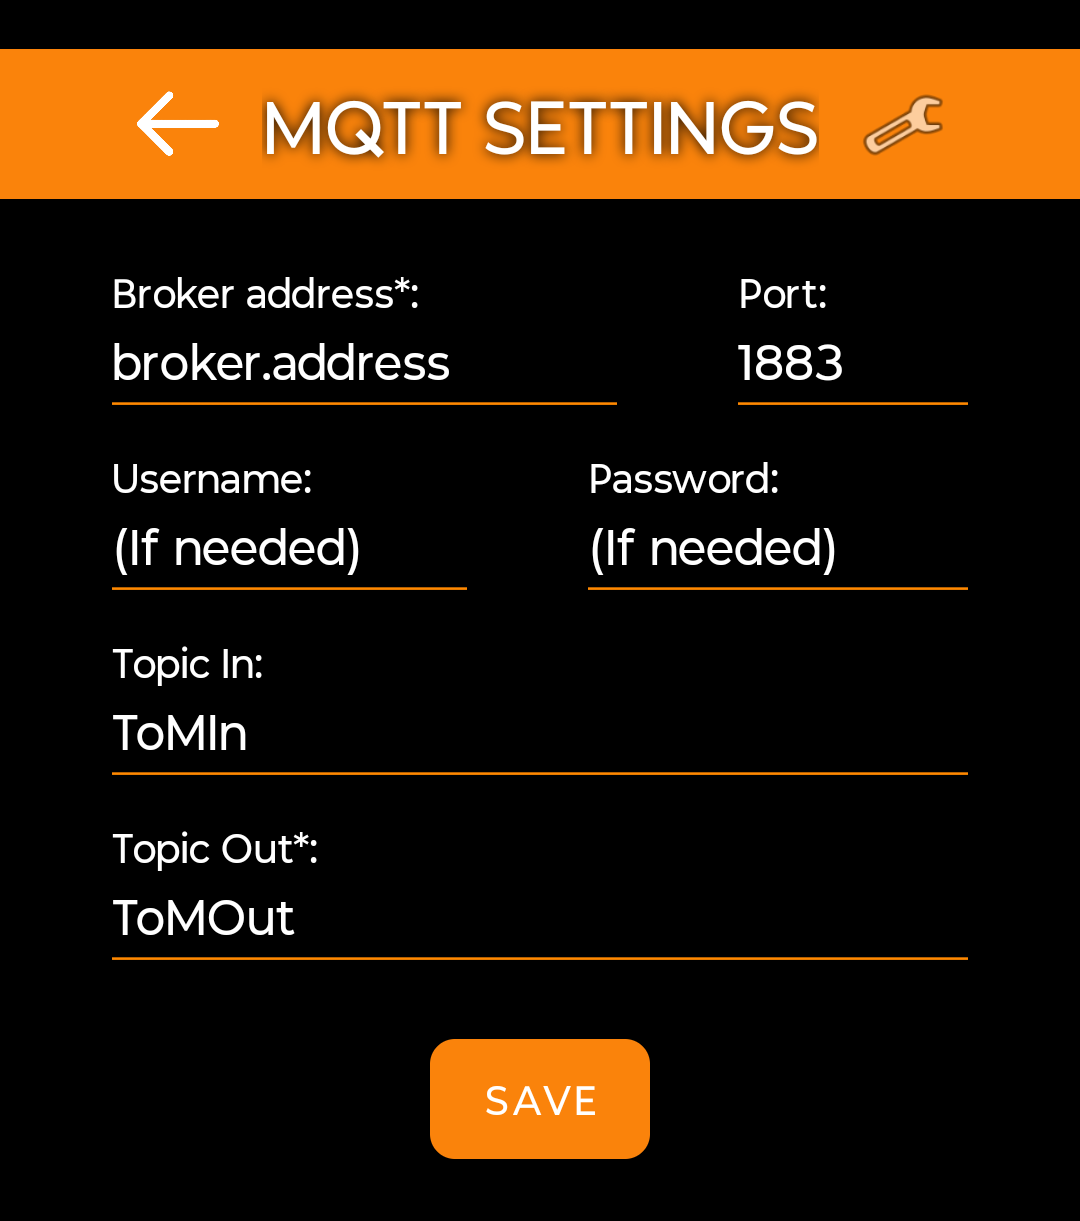
\includegraphics[width=0.65\textwidth]{figures/tom_app_settings.png}
    \caption{Einstellungsseite der ToM+-Android-App}
\end{figure}

\subsection{Kurzer Überblick über den Verbrauch}

ToM wird die 12-V-Batteriestromversorgung nutzen, die direkt vom OBD-Stecker bezogen wird, und
verbraucht dabei nicht viel Strom, wie die folgenden Messwerte zeigen.

\begin{figure}[H]
    \centering
    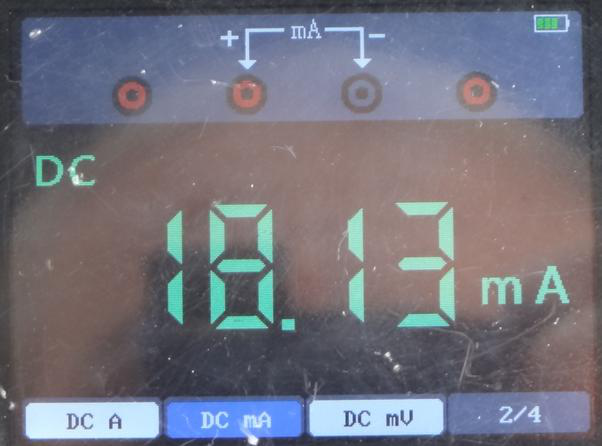
\includegraphics[width=0.65\textwidth]{figures/consumption_off.png}
    \caption{Stromverbrauch bei ausgeschaltetem Twizy}
\end{figure}

Wenn die Hauptplatine aktiv ist und das Display eingeschaltet ist, beträgt der Stromverbrauch etwa 90 mA. Ist zudem das WLAN aktiviert, liegt der Stromverbrauch in etwa bei dem unten angegebenen Wert (möglicherweise etwas höher aufgrund der letzten Updates, mit denen die 3D-Grafik eingeführt wurde).

\begin{figure}[H]
    \centering
    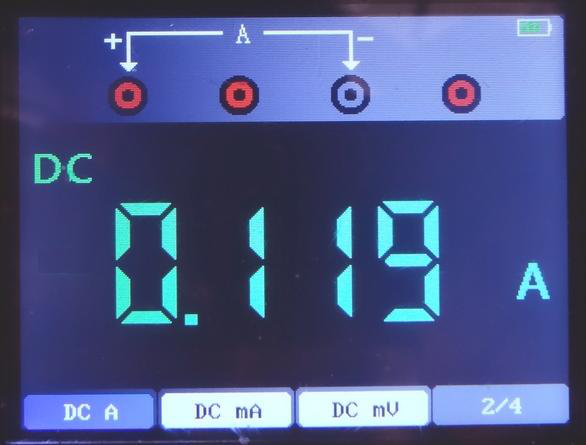
\includegraphics[width=0.65\textwidth]{figures/consumption_on_wifi.png}
    \caption{Stromverbrauch bei eingeschaltetem ToM+ mit WLAN}
\end{figure}

Wenn der Twizy ausgeschaltet ist, wechselt die Blackbox in den Ruhemodus und verbraucht 18 mA.
Darüber hinaus ermöglicht Ihnen die Touch-Funktion eine wesentlich einfachere Interaktion mit dem
Gerät und dessen LCD-Display. Da es eine resistive Touch-Technologie verwendet, können Sie  Ihre
Finger oder einen kleinen Stylus-Stift aus hartem Kunststoff verwenden, um die Tasten zu betätigen. Es ist zwar nicht so leistungsstark wie
  Armaturenbretter mit kapazitivem Touchscreen, aber sobald Sie es einmal ausprobiert haben, werden Sie nicht mehr darauf verzichten wollen, 
  glauben Sie mir!

\clearpage

\section{Mitgeliefertes ToM+-Kit}

Beim Versand wird das ToM+ in der Regel in einem braunen Karton verpackt, um die internen Platinen
und Sensoren vor Stößen während des Transports zu schützen. In dieser neueren Version sind keine langen Kabel mehr erforderlich, sondern lediglich ein kürzeres, das an die interne ToM+-Hauptplatine angeschlossen ist und in einem kleinen schwarzen Kunststoffgehäuse
untergebracht ist, das ich gewöhnlich als „Black Box“ bezeichne. Selbstverständlich ist auch das resistive LCD-Touchdisplay im Lieferumfang enthalten, auf dem Sie alle Funktionen anzeigen und konfigurieren können.
Es sind keine Schrauben oder Klebeband mehr erforderlich! Nur ein einfaches Clip-Display, das direkt auf das ursprüngliche Armaturenbrett passt.

\begin{figure}[H]
    \centering
    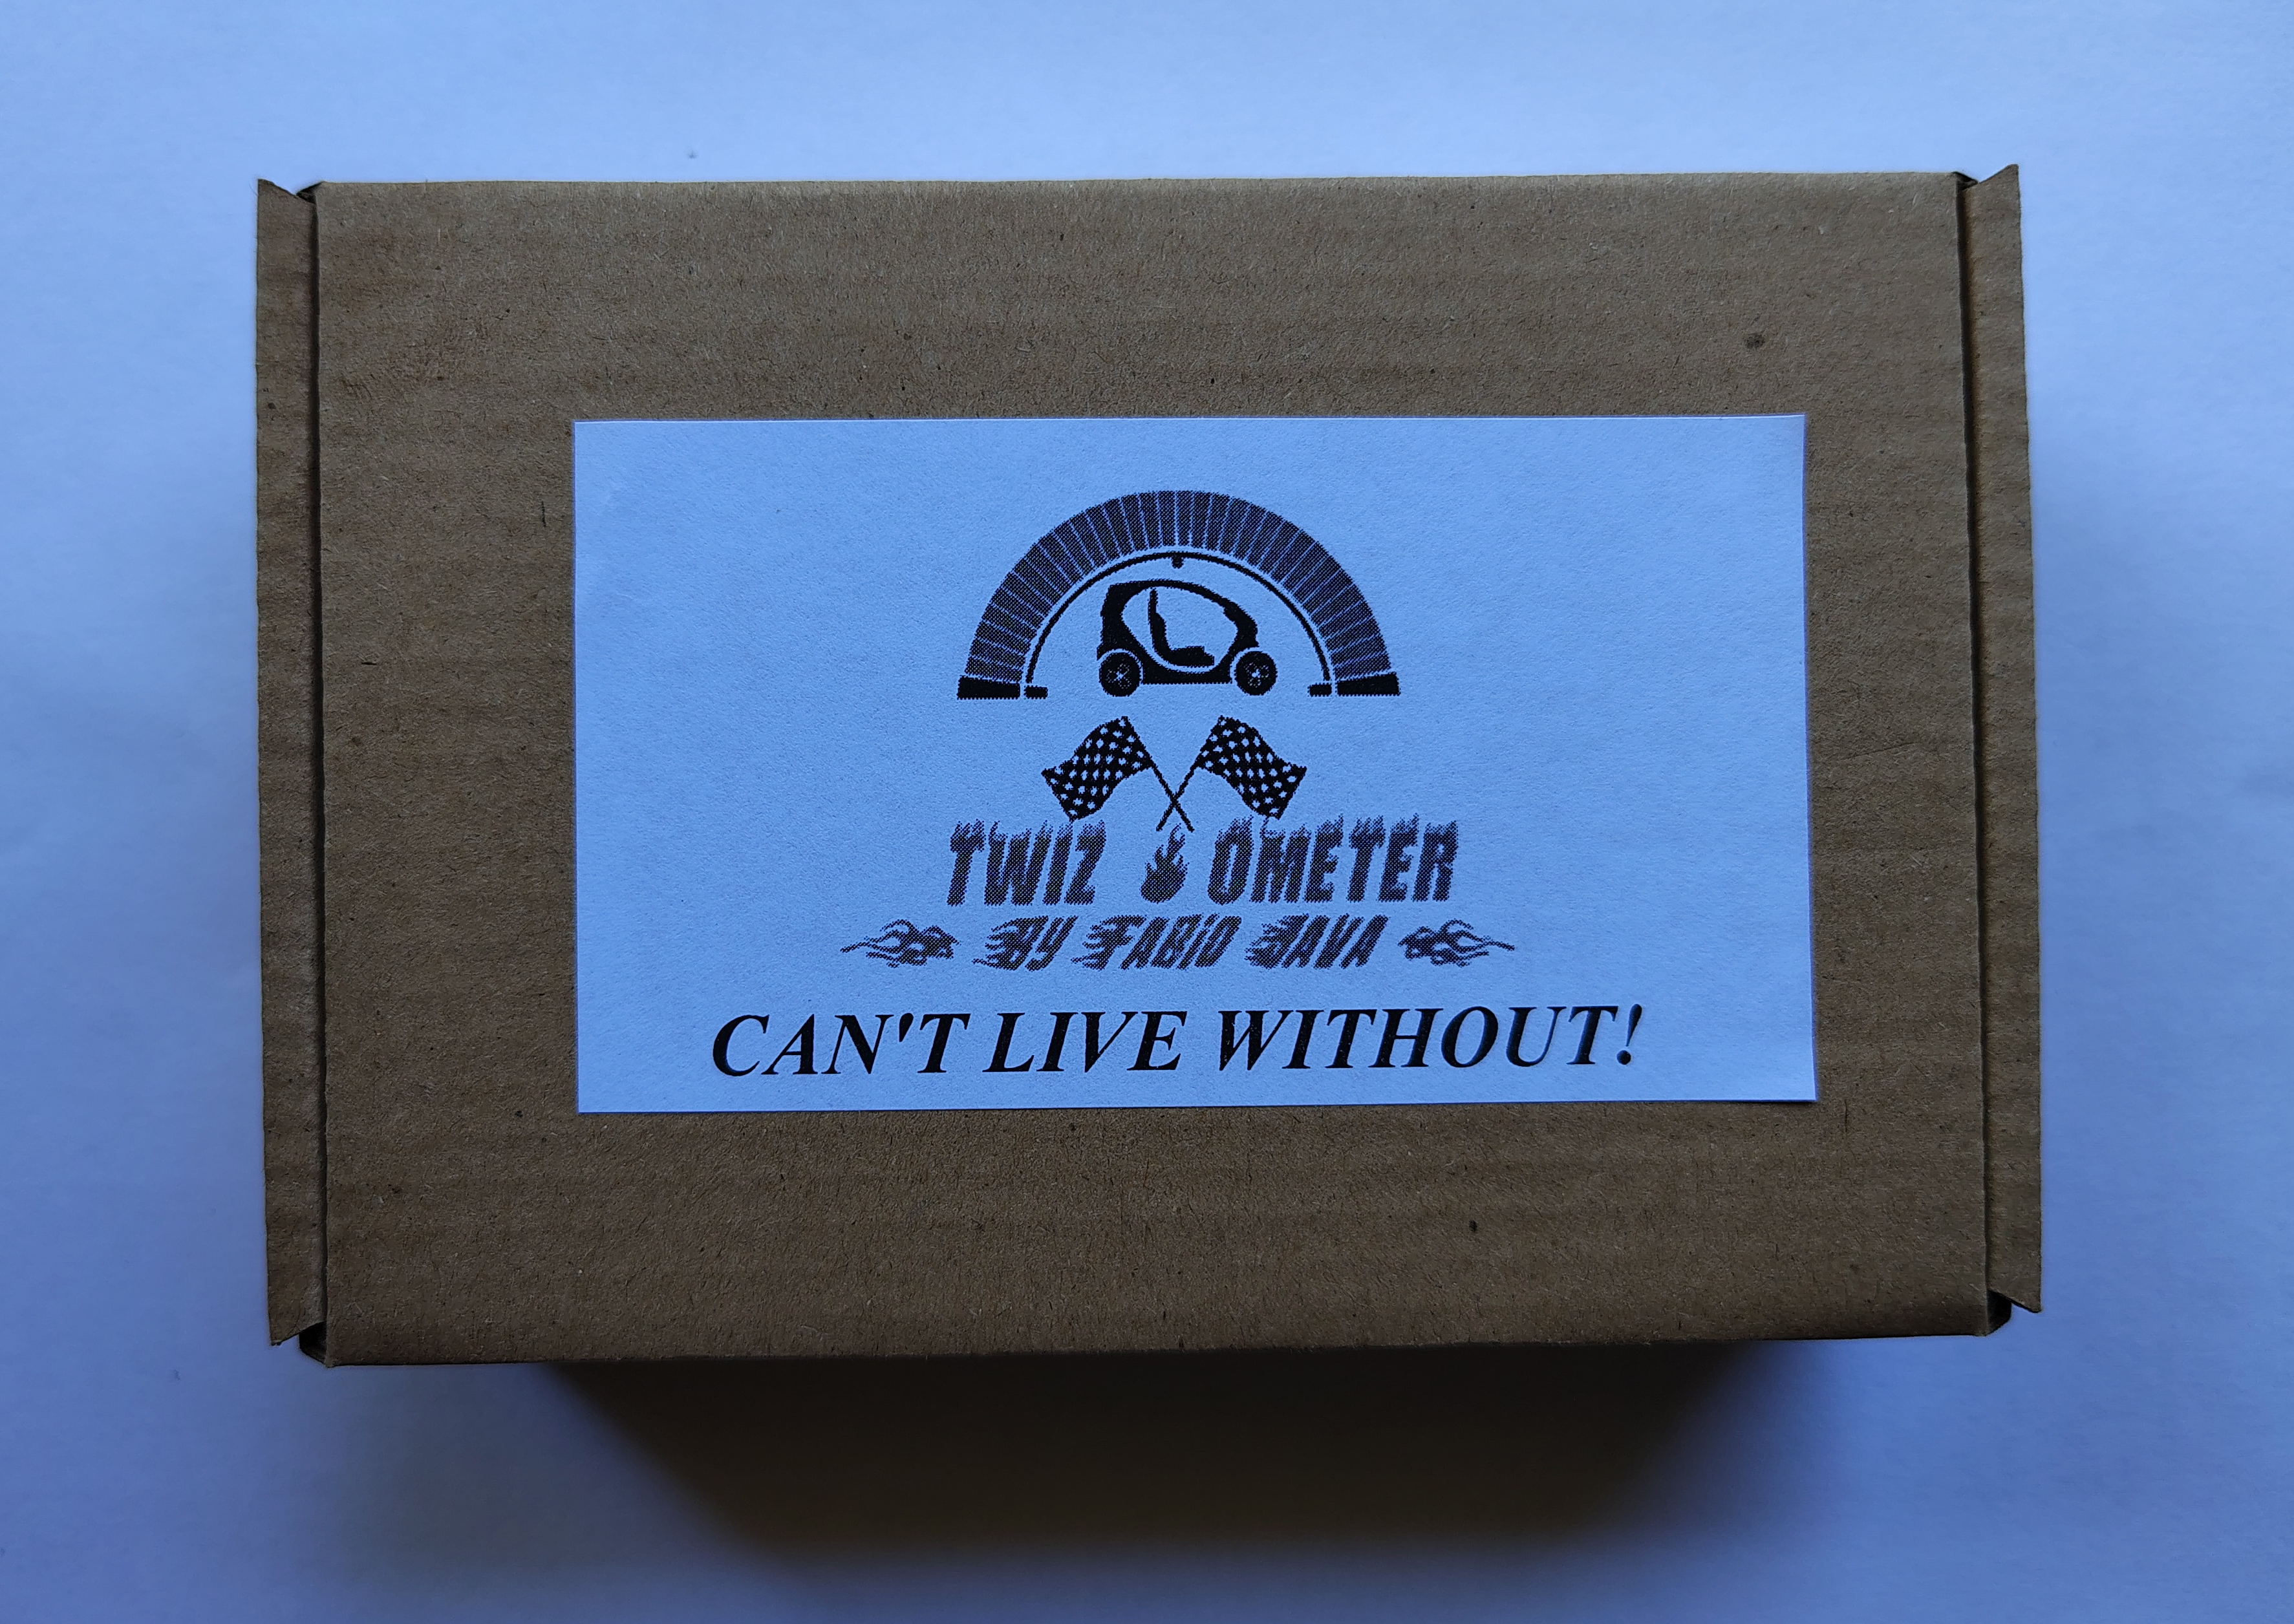
\includegraphics[width=0.8\textwidth]{figures/box.png}
    \caption{Mitgeliefertes ToM+-Kit}
\end{figure}

\subsection{Die Black Box}

Die Black Box ist die Hauptplatine von ToM+ und enthält die meisten Komponenten, die
für den Betrieb des Systems erforderlich sind. Sie bietet:
\begin{itemize}
    \item Einen externen Anschluss für das LCD-Display;
    \item einen Erweiterungsanschluss mit Strom- und GPIO-Pins;
    \item eine integrierte OBD-Buchse für den Twizy-CAN-Bus;
    \item einen Micro-USB-Anschluss für Firmware-Updates;
    \item eine Buchse für den Schalter am Scheibenwischerhebel;
    \item einen ToM+-Ein-/Aus-Schalter
\end{itemize}

\begin{figure}[H]
    \centering
    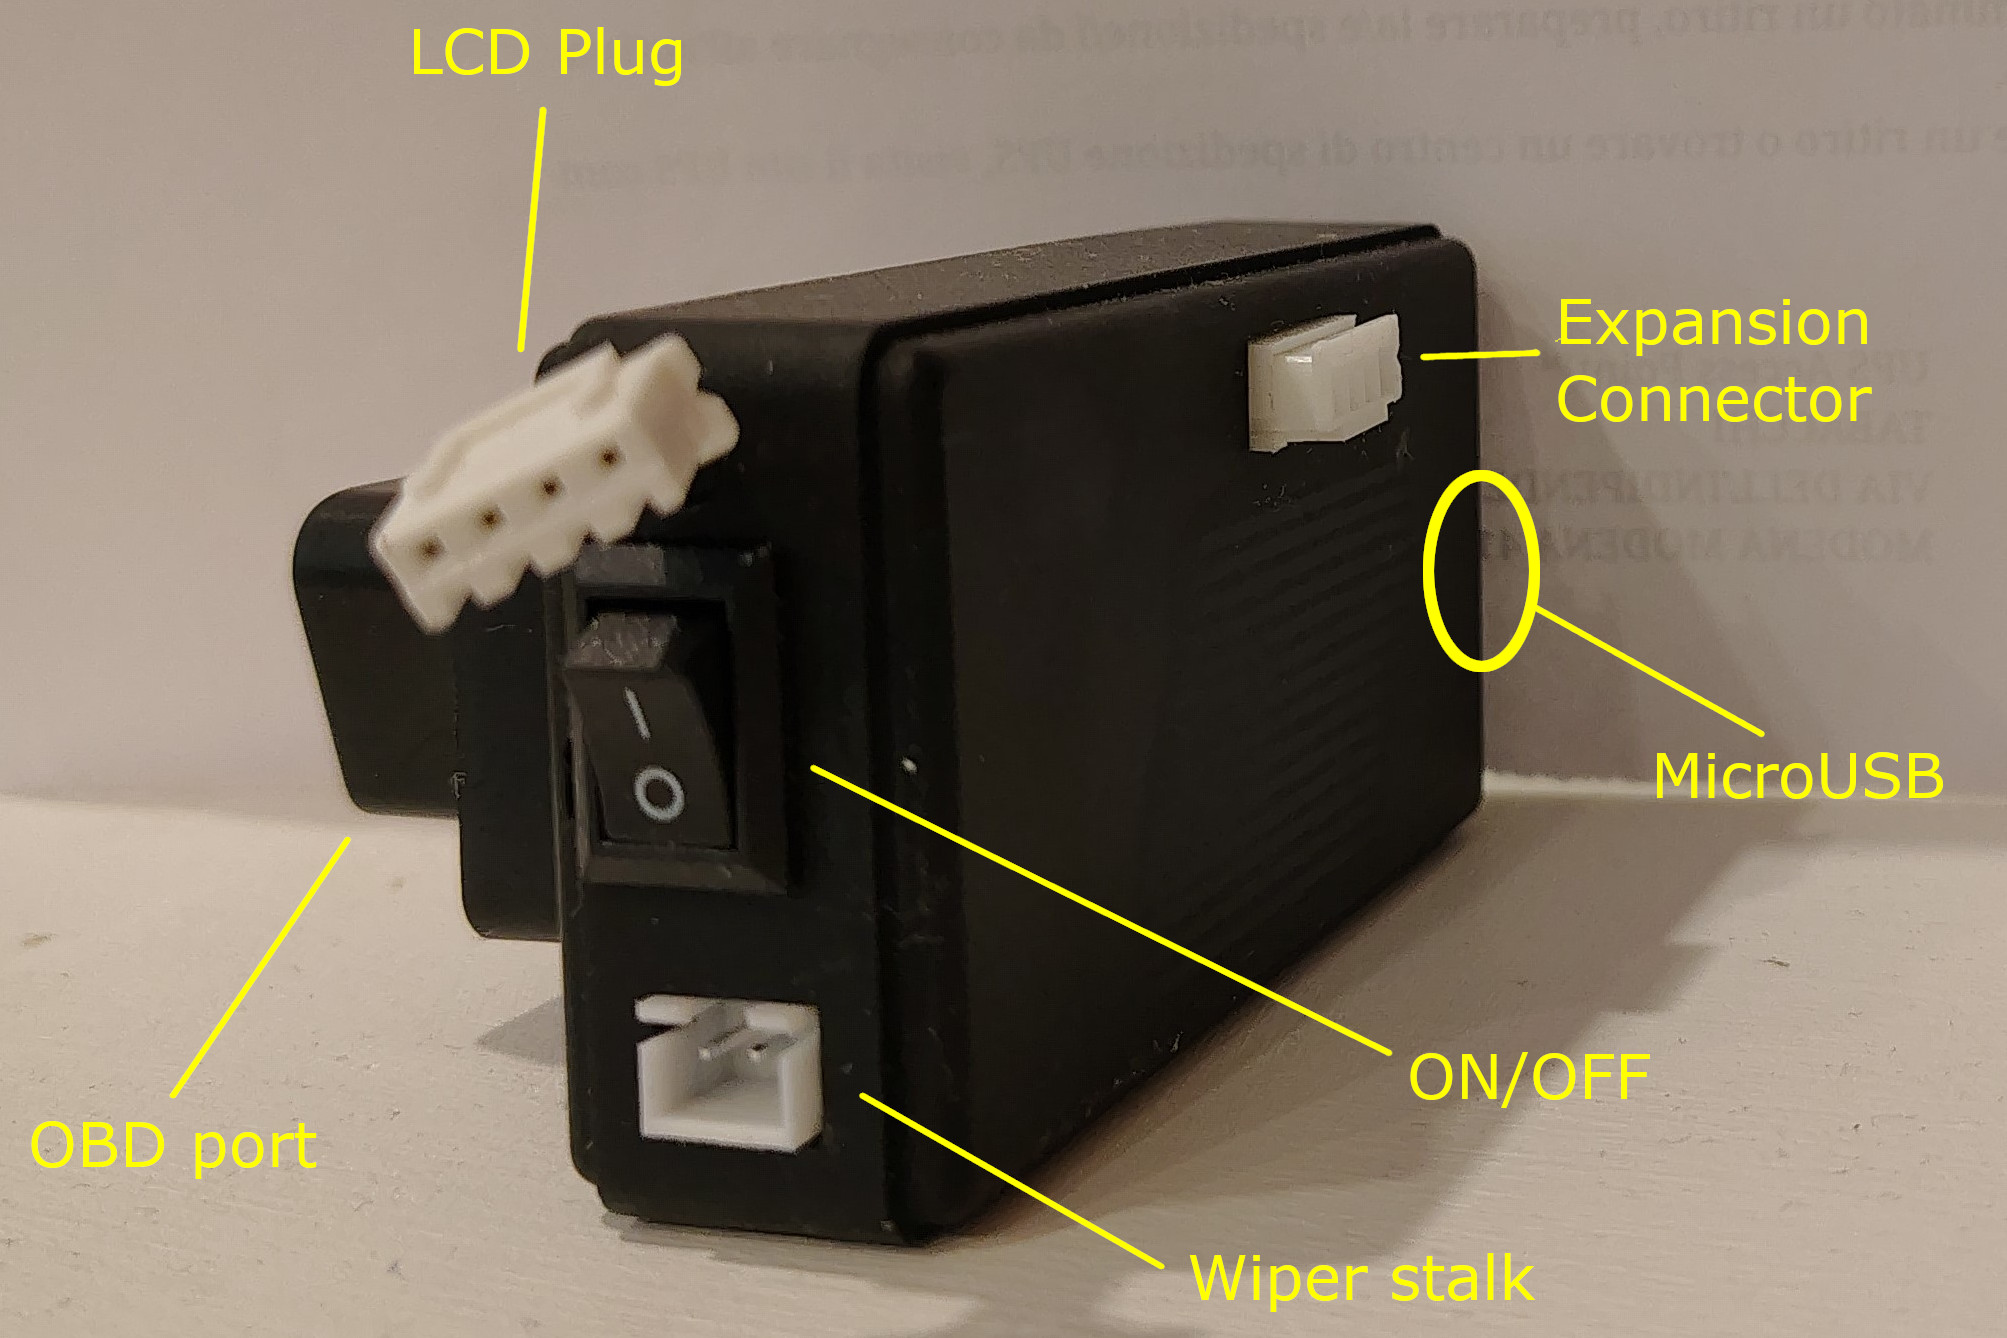
\includegraphics[width=0.75\textwidth]{figures/black_box.jpg}
    \caption{Die Blackbox}\label{fig:blackbox_components}
    \end{figure}

\subsection{Der Erweiterungsanschluss}

Wenn Sie Ihr ToM+ weiter anpassen möchten, können Sie dies ganz einfach über den
hier abgebildeten Anschluss tun. Tatsächlich stellt er eine zusätzliche 5-V-Stromversorgung bereit, die von
VCC (ehemals rotes Kabel) und GND (ehemals schwarzes Kabel) stammt, sodass Sie eine externe LED, einen
kleinen Summer oder was auch immer Sie wünschen, mit Strom versorgen können. Die beiden anderen Kabel sind allgemeine Ein- und Ausgangs-Pins:
PIN1 (ehemals gelb) und PIN2 (ehemals blau). Sie können entweder als Ein- oder als Ausgang dienen, je nachdem, welche Einstellung Sie auf der \textit{„Erweiterungsseite“} des ToM-\textbf{Webservers} wählen. In dieser neuesten Version des Geräts ist der Erweiterungsstecker in die schwarze Box integriert (ohne farbige Kabel), die Pinbelegung bleibt jedoch unverändert.
Denken Sie daran, vor der Verwendung die Schutzabdeckung zu entfernen und eine Eingangsspannung von \textbf{maximal 3,3 V} zu verwenden. Bei höheren
Spannungen müssen Sie einen geeigneten Widerstandsteiler vorsehen.

\begin{figure}[H]
    \centering
    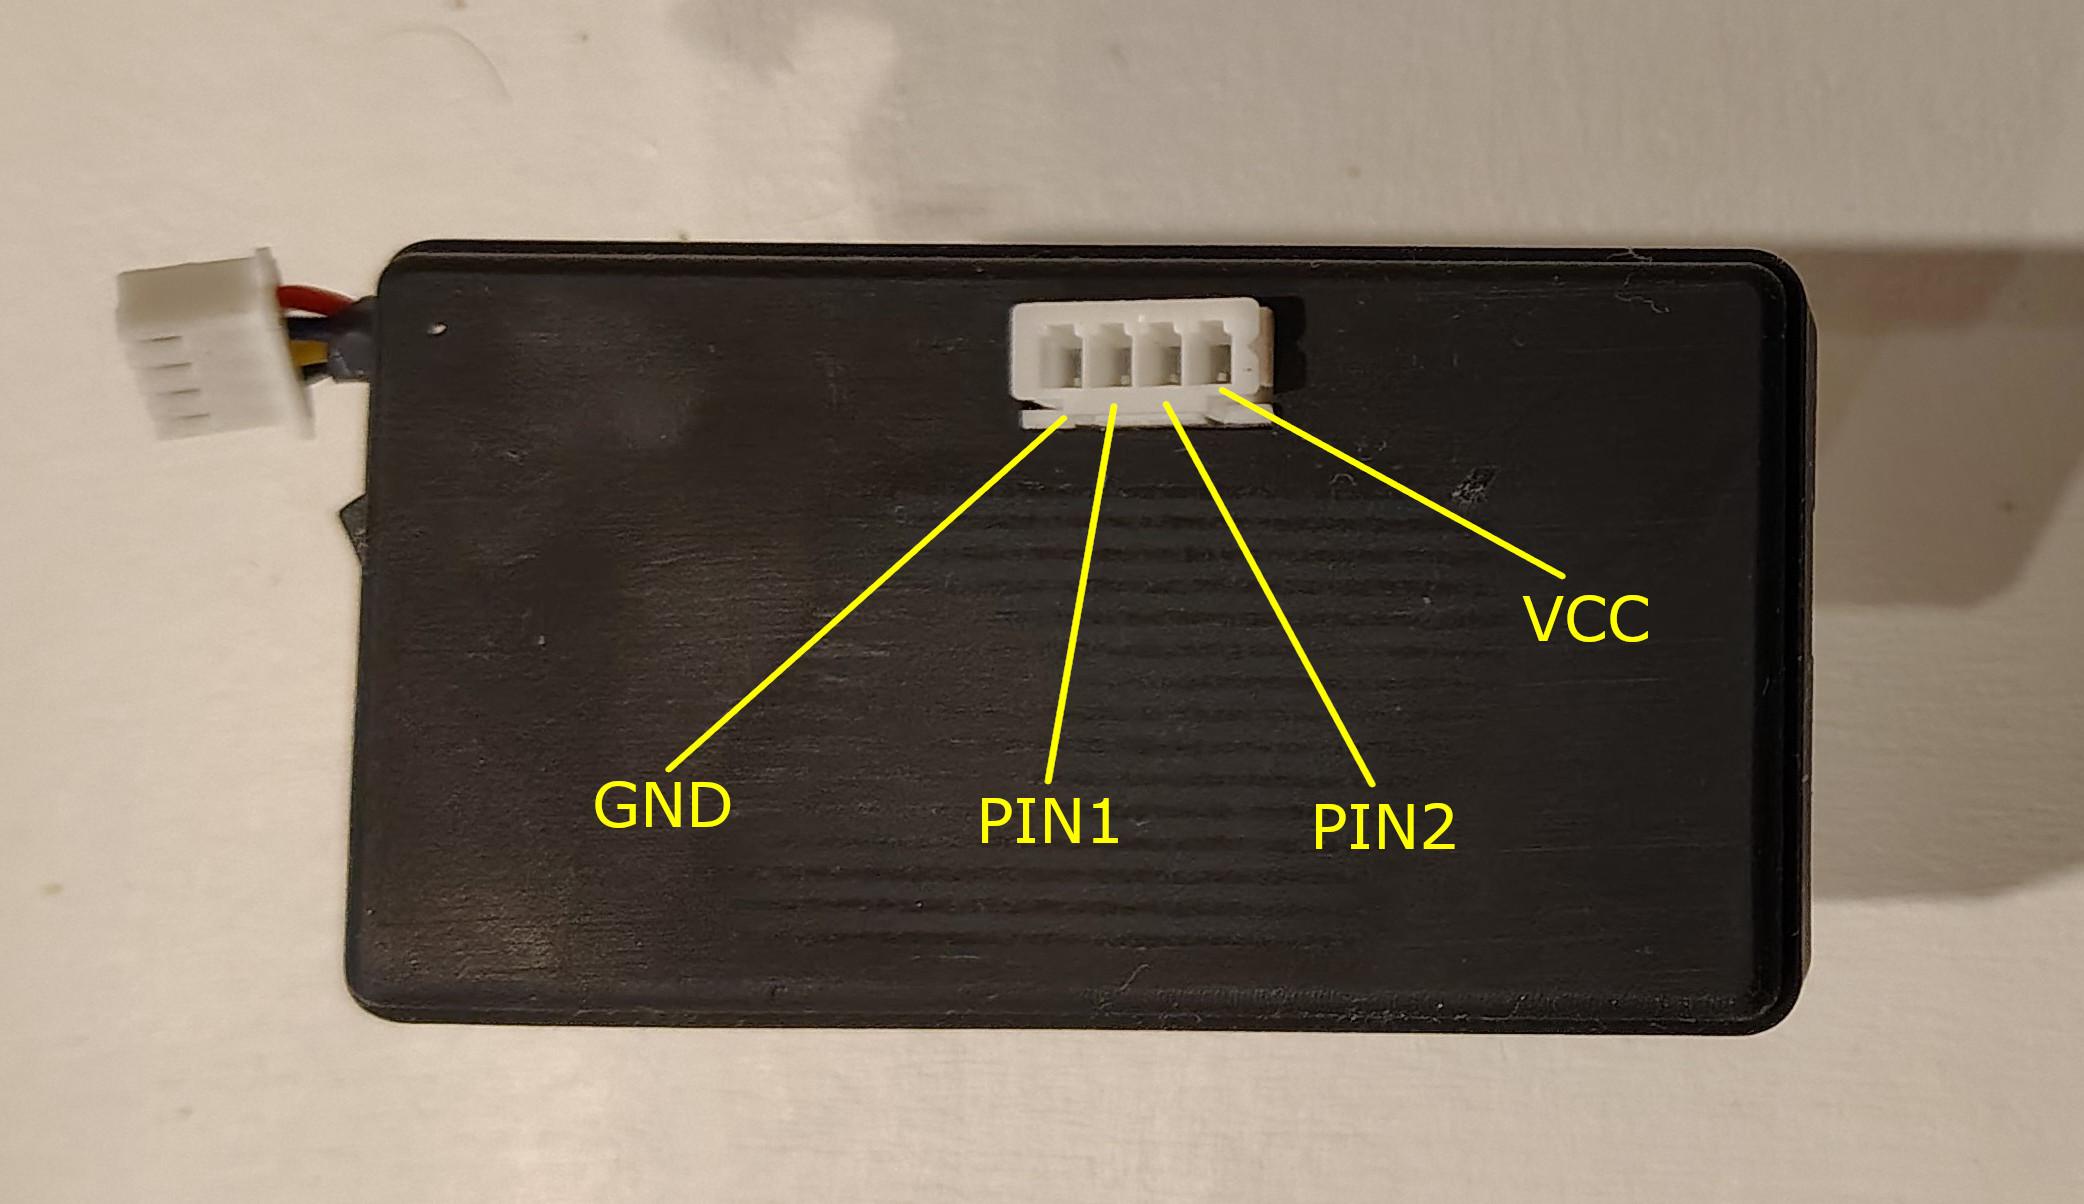
\includegraphics[width=0.7\textwidth]{figures/expansion_bb.jpg}
    \caption{Erweiterungsstecker}\label{fig:expansion_pinout}
    \end{figure}

\subsection{Das LCD-Display und der Ständer}

Das resistive Touch-LCD-Display ist in einen 3D-gedruckten Ständer eingebettet, der auf das Original-Armaturenbrett aufgesteckt wird. Auf Wunsch erhalten Sie auch eine eigenständige 3D-Halterung, mit der Sie das Display wie das Standard-ToM am Handschuhfach befestigen können. Auf diese Weise verfügen Sie über ein 2-in-1-Gerät, das je nach Wunsch sowohl aufsteckbar als auch eigenständig genutzt werden kann. Ein microSD-Steckplatz steht für Firmware-Updates zur Verfügung.

\begin{figure}[H]
    \centering
    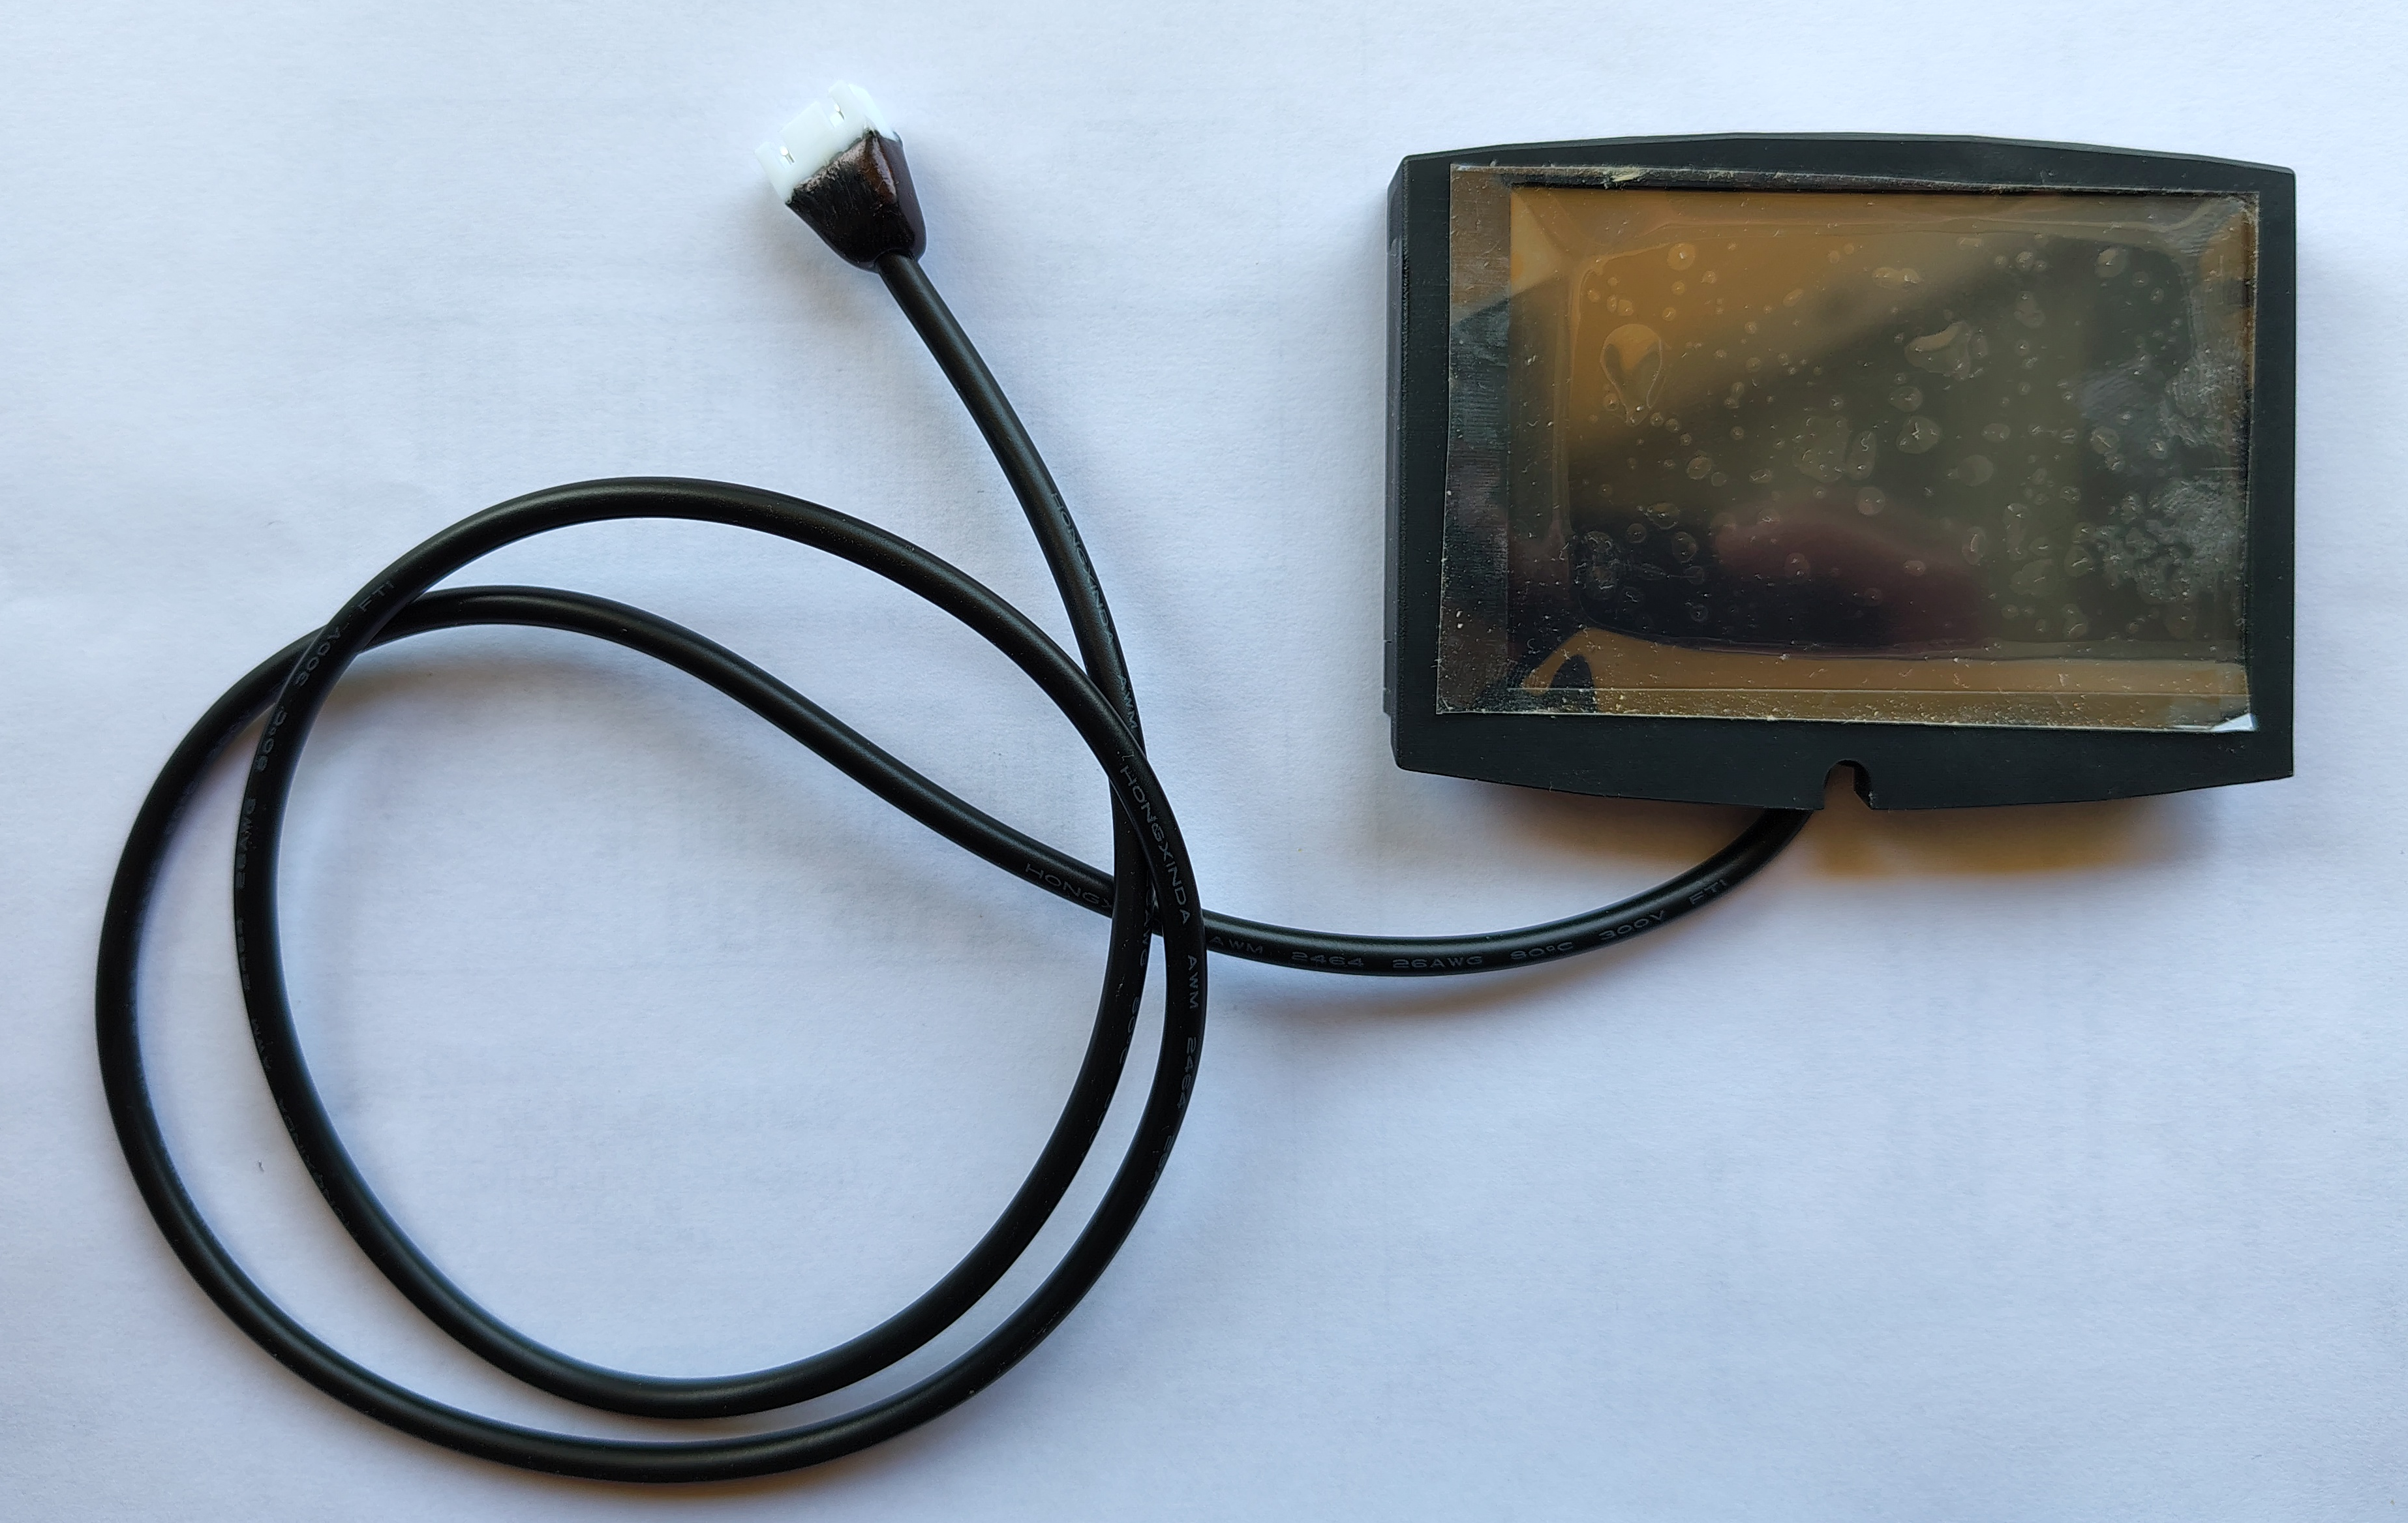
\includegraphics[width=0.8\textwidth]{figures/display.png}
    \caption{LCD-Display zum Aufstecken}
\end{figure}

Das Display, das wie auf den Abbildungen zu sehen mit einer Schutzfolie versehen ist, lässt sich in die 3D-Halterung einsetzen, sodass Sie über einen verstellbaren Ständer verfügen, den Sie an einer beliebigen Stelle platzieren können.

\begin{figure}[H]
    \centering
    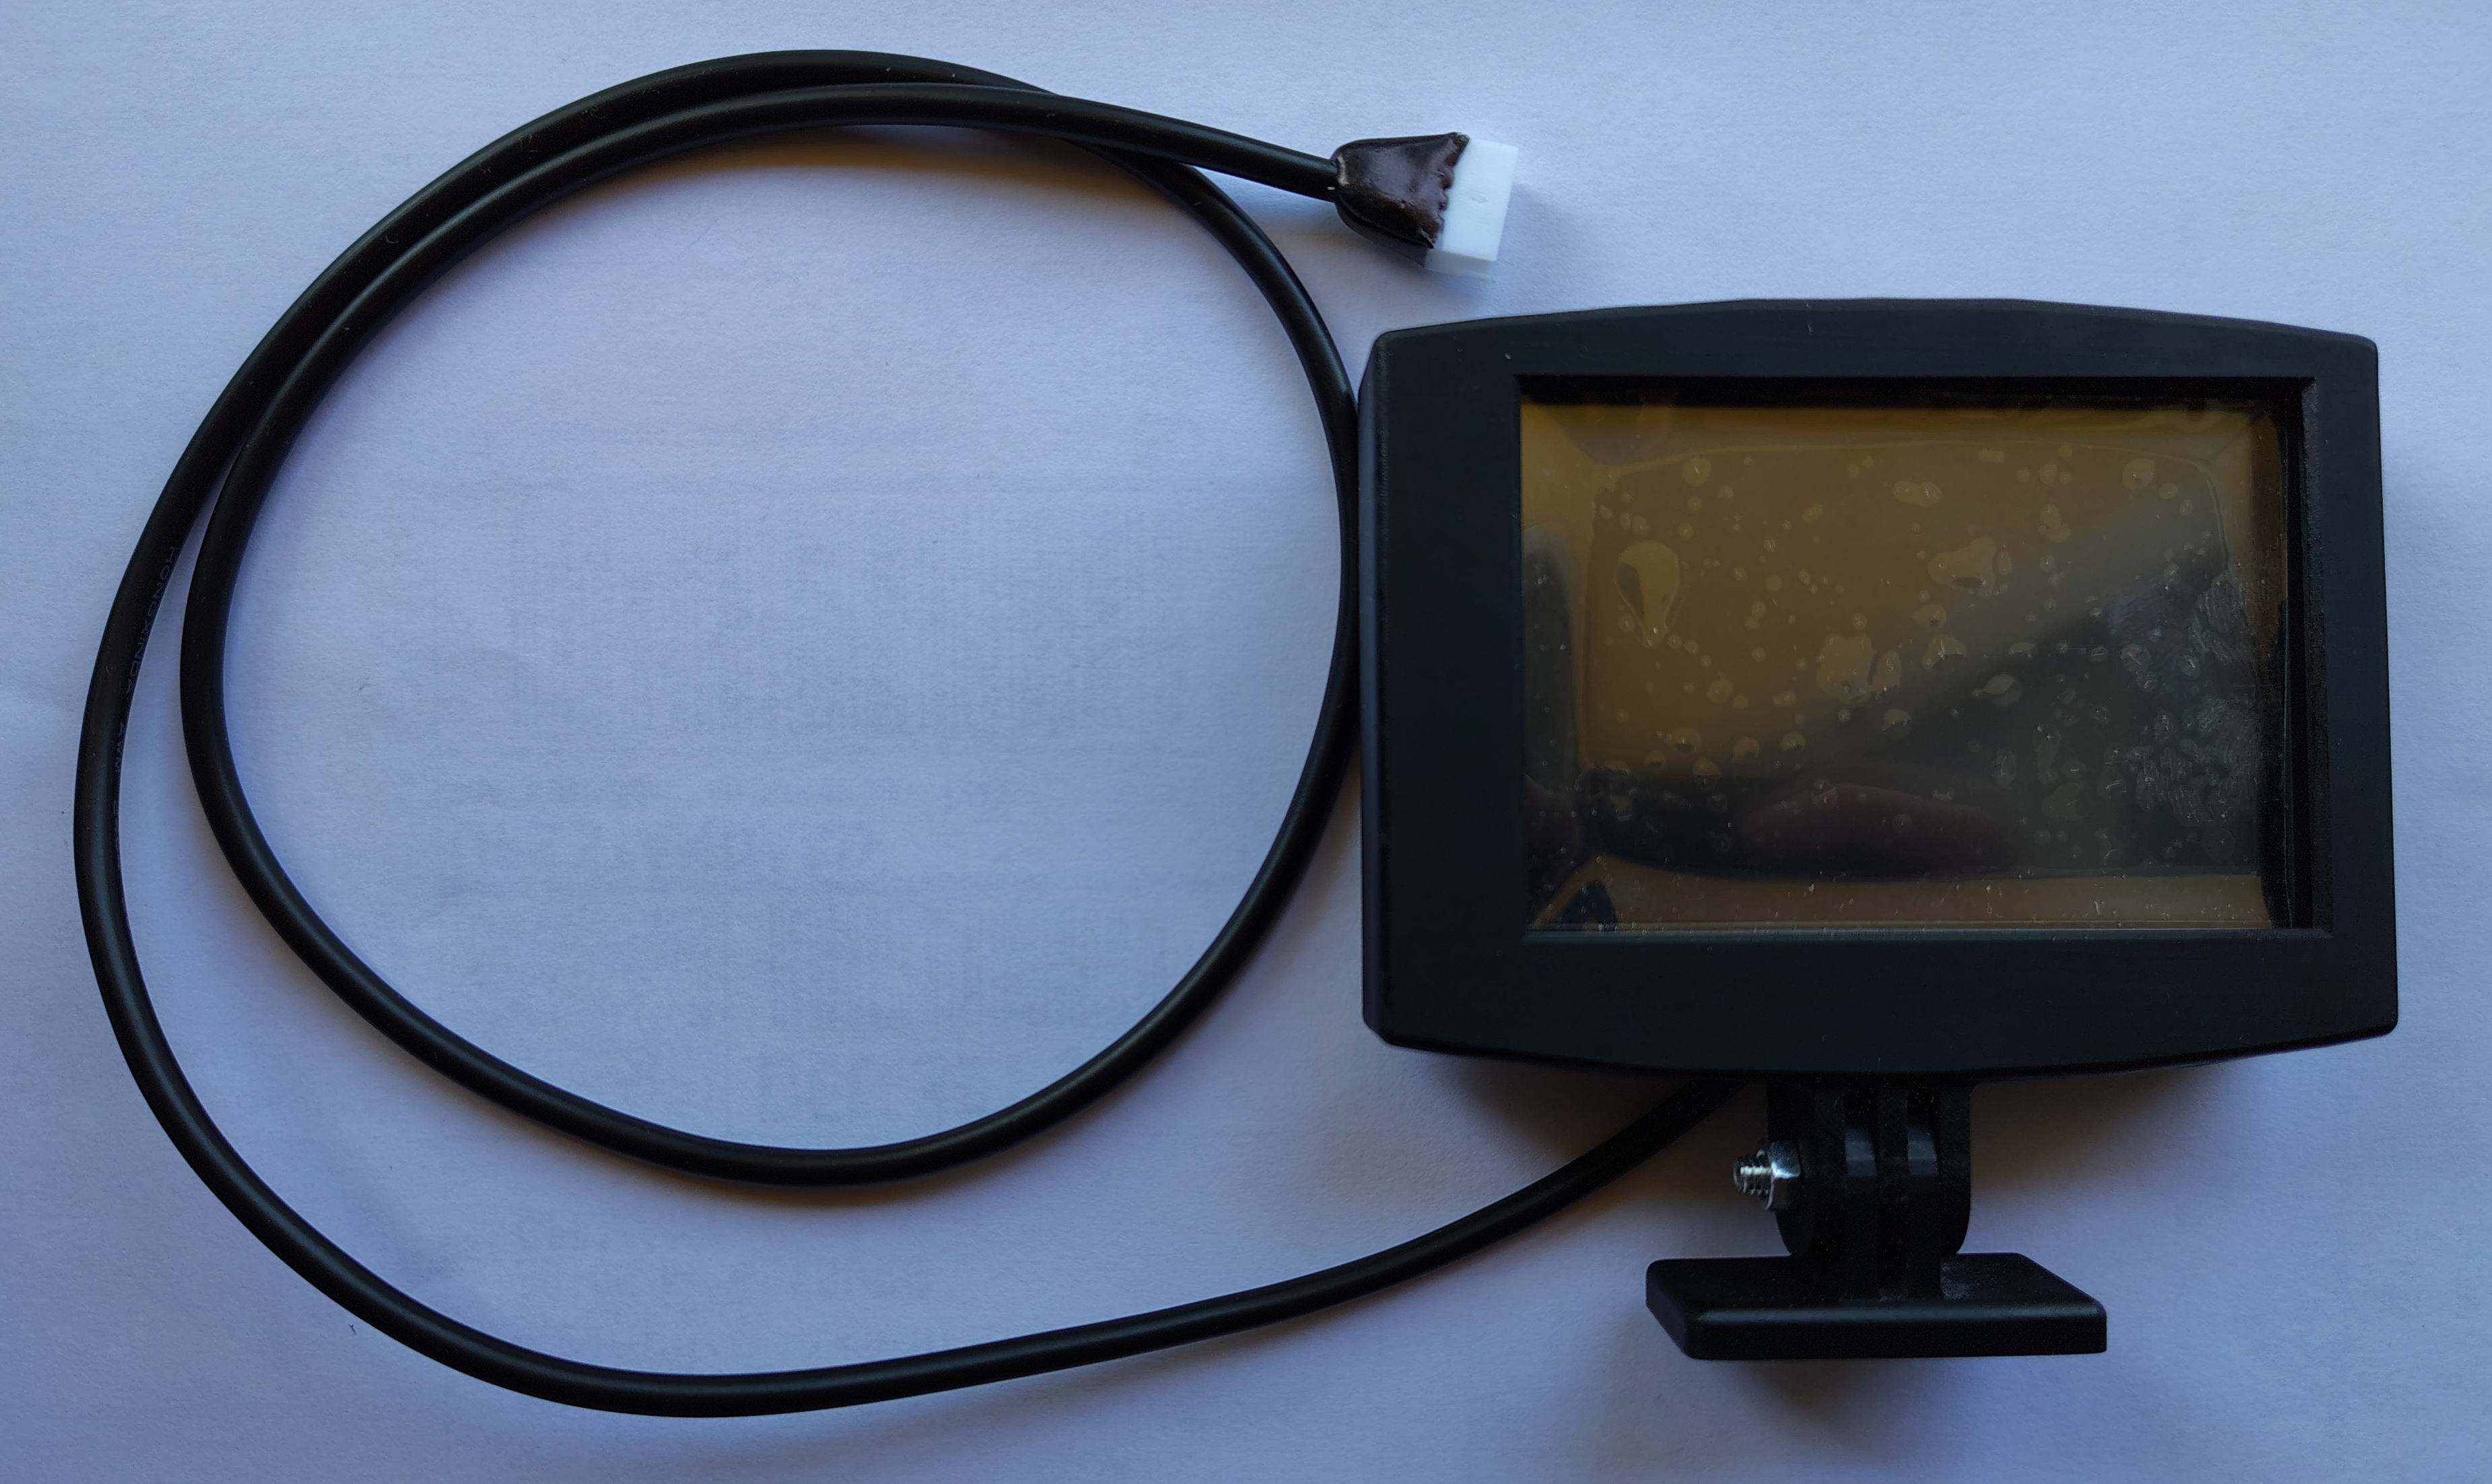
\includegraphics[width=0.8\textwidth]{figures/3d_stand_wdisplay.png}
    \caption{LCD-Display als eigenständiges Gerät}
\end{figure}

In der eigenständigen Version können Sie es mit der Abdeckung und den Schrauben befestigen, die Sie zusammen mit dem faltbaren 3D-Ständer im Lieferumfang finden, wie auf den folgenden Abbildungen gezeigt.

\begin{figure}[H]
    \centering
    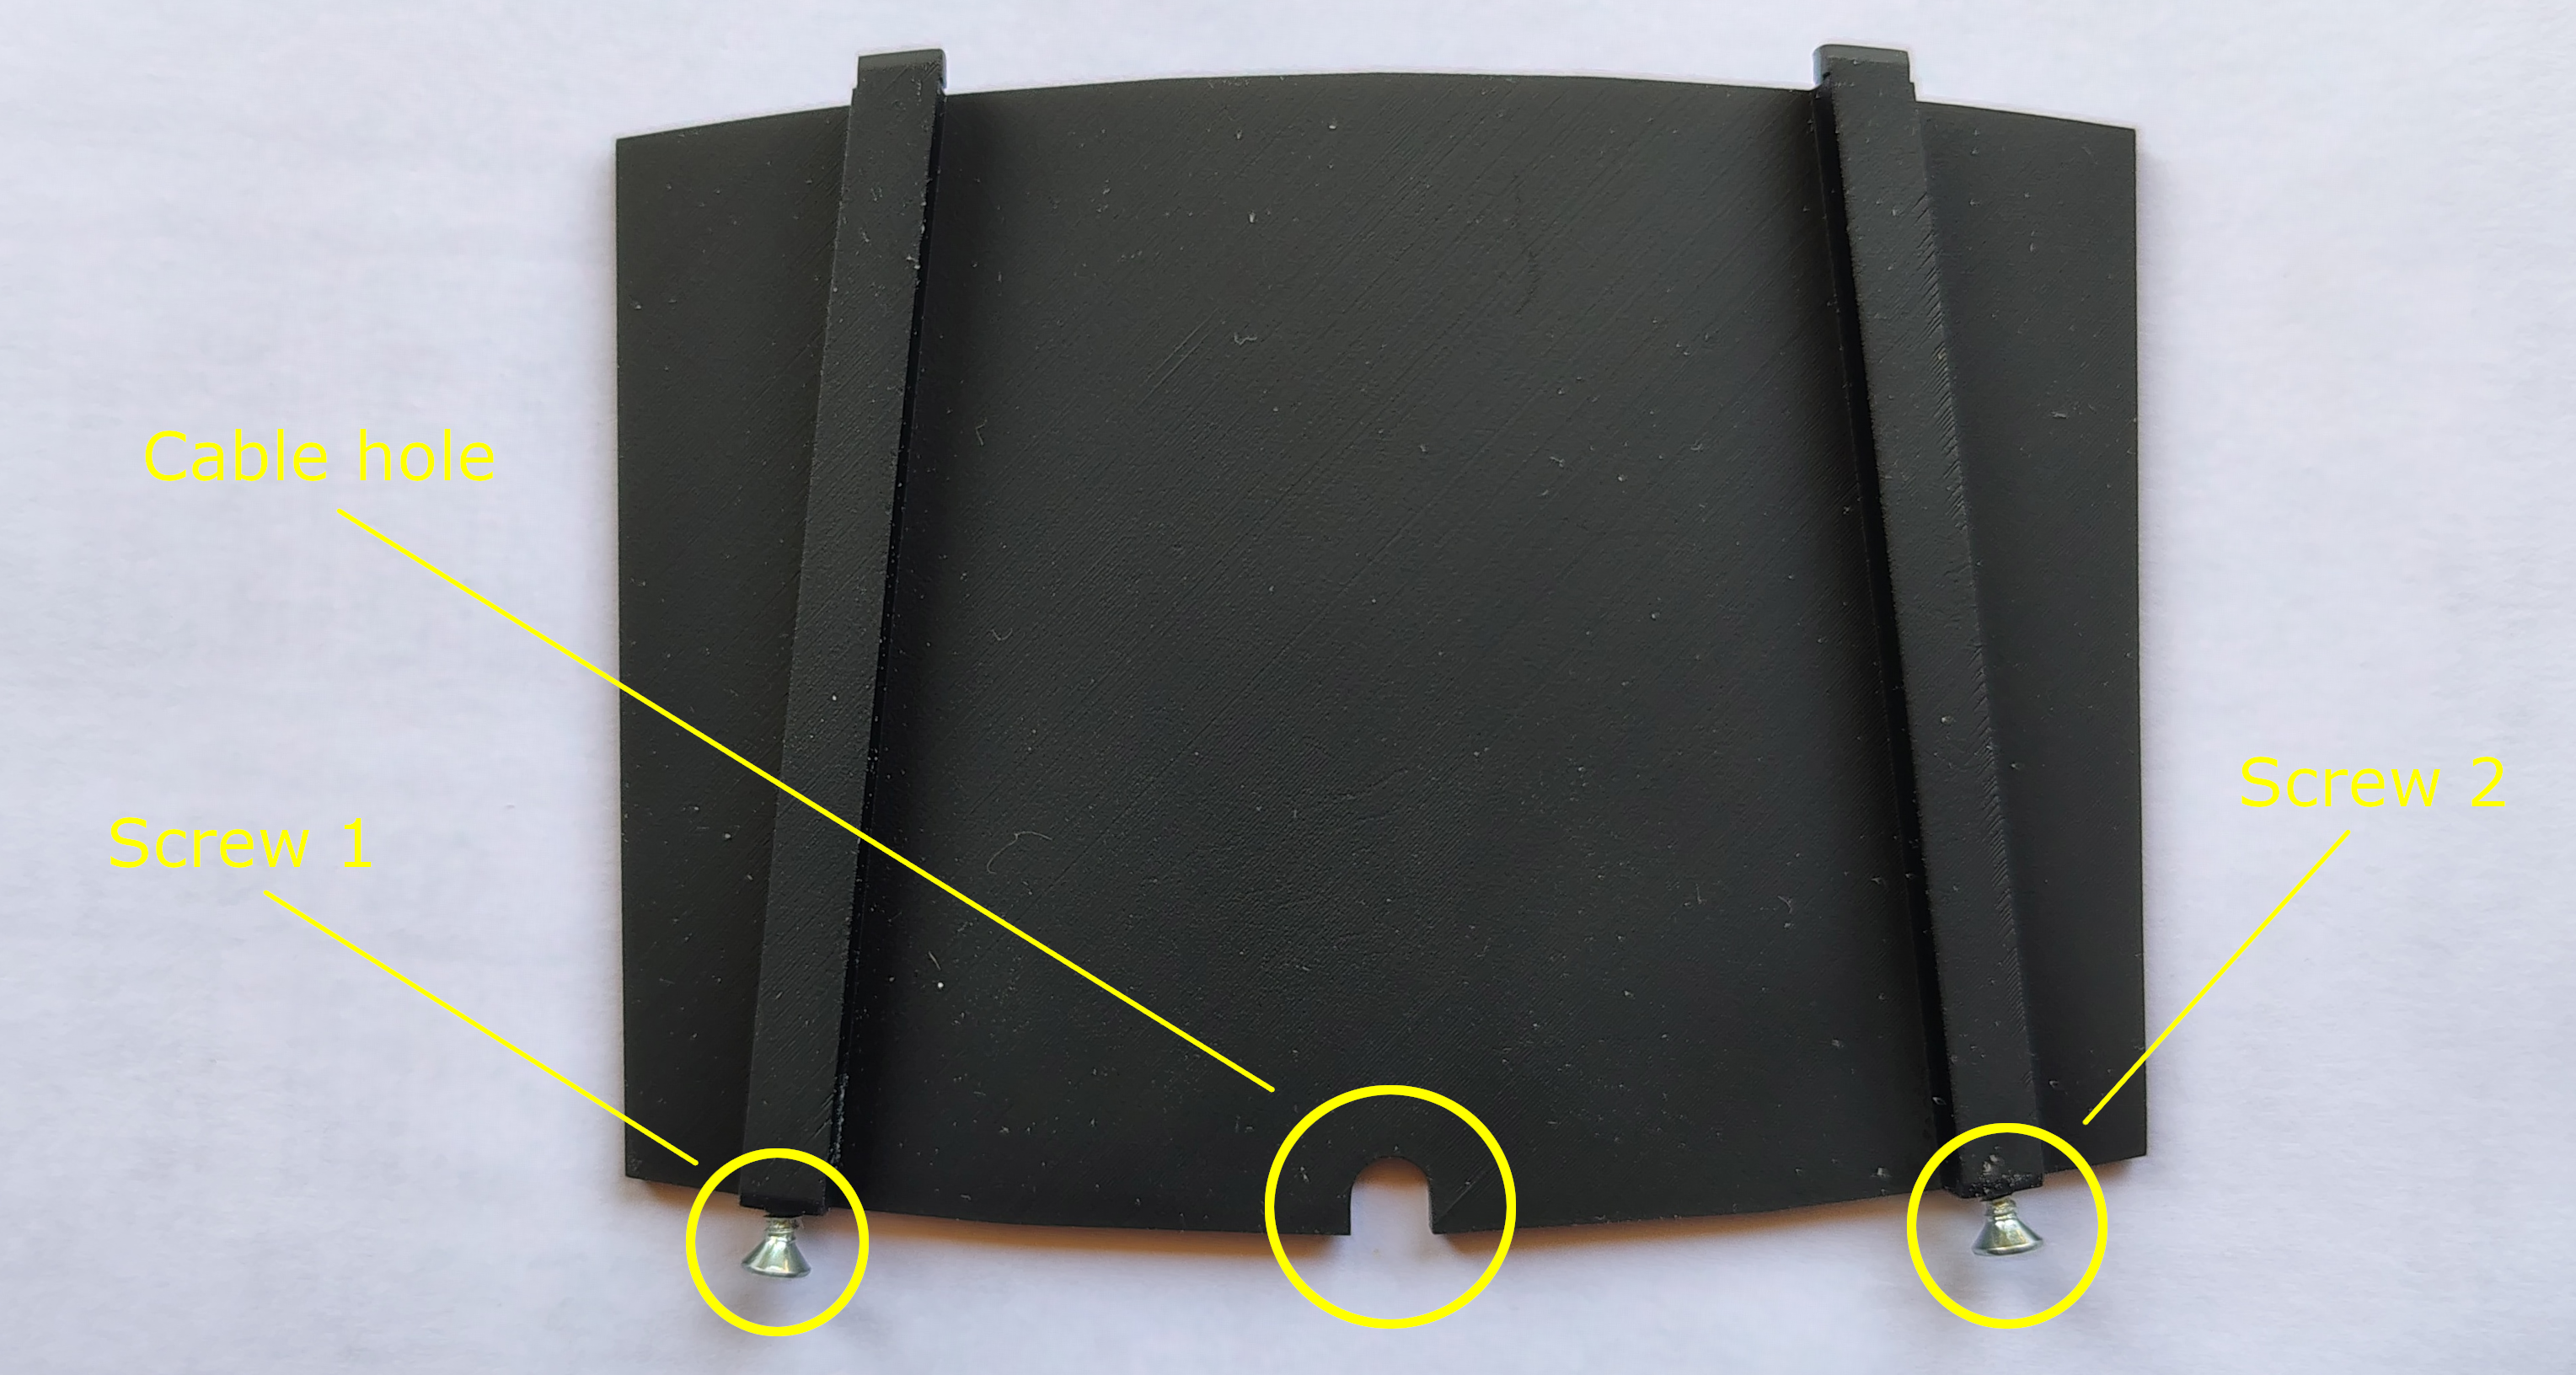
\includegraphics[width=0.8\textwidth]{figures/back_cover.png}
    \caption{Mitgelieferte LCD-Abdeckung}\label{fig:back_cover}
    \end{figure}

Der 3D-Ständer verfügt außerdem über Löcher an der Basis, falls Sie ihn am Handschuhfach befestigen möchten. Die weiteren Löcher am Rahmen dienen zur Befestigung der hinteren Abdeckung, um das Display im Inneren an Ort und Stelle zu halten.

\begin{figure}[H]
    \centering
    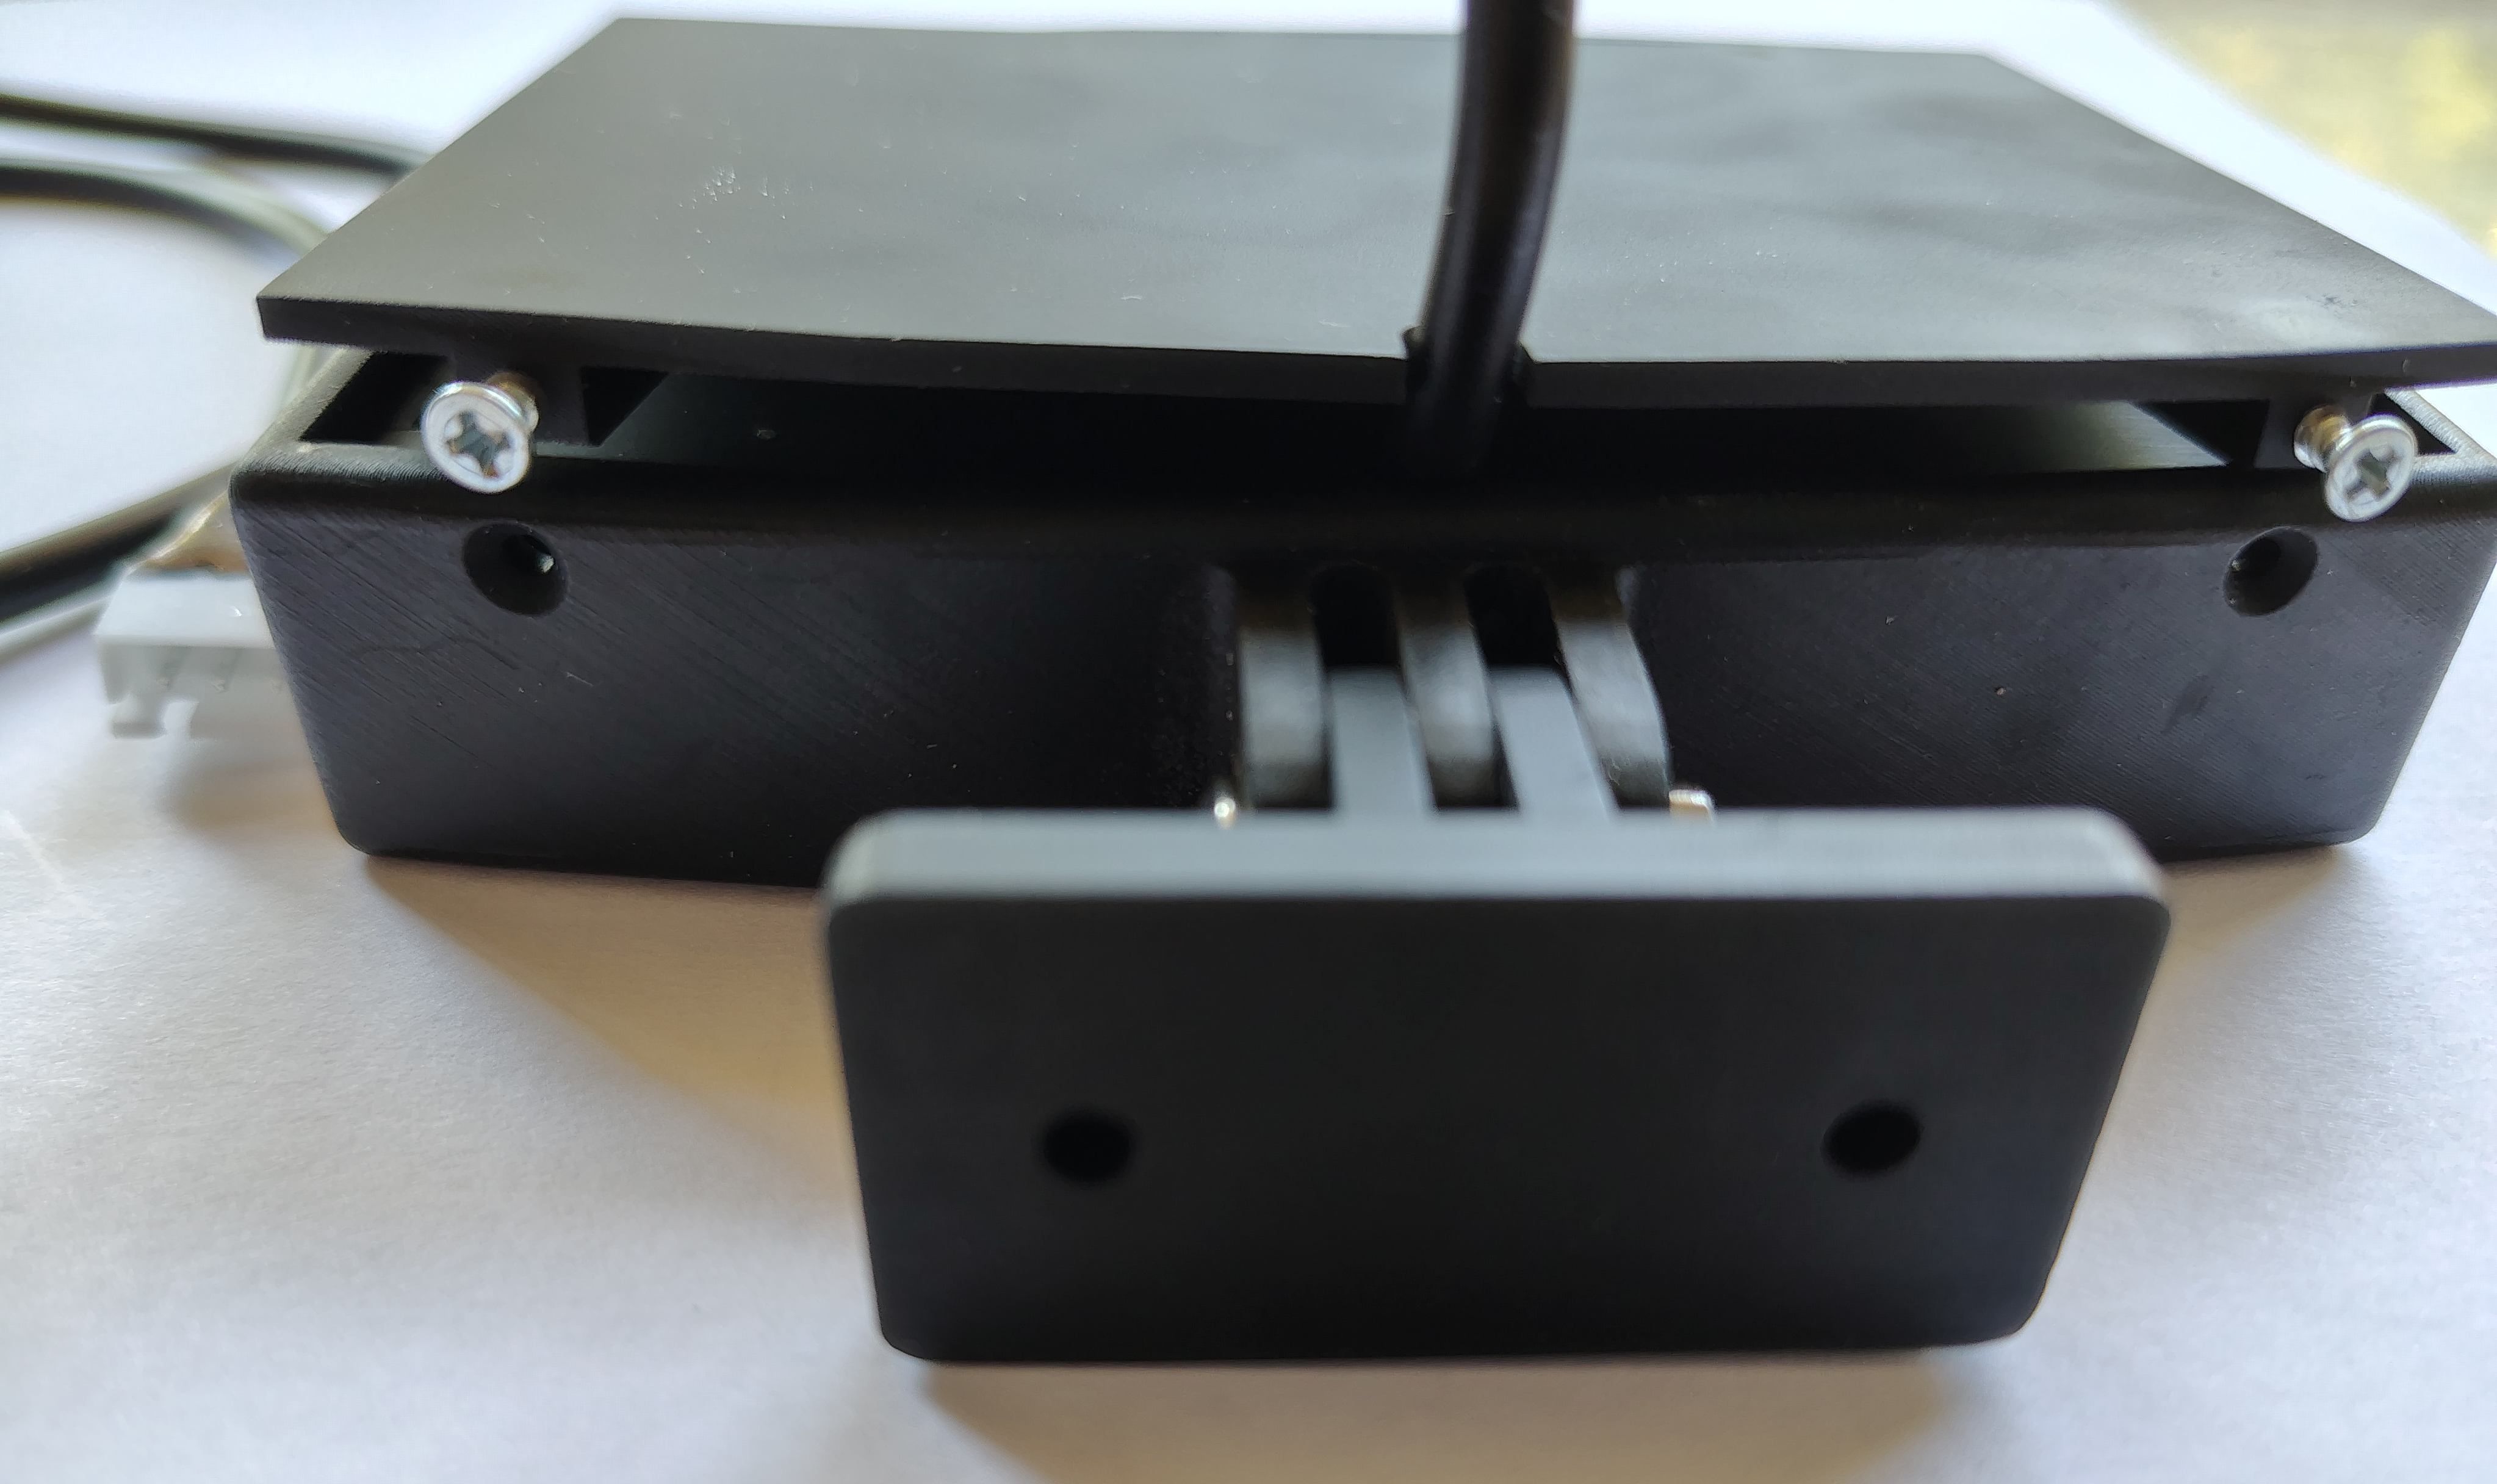
\includegraphics[width=0.8\textwidth]{figures/bottom_cover_screwholes.png}
    \caption{Schraubbefestigung der LCD-Abdeckung}\label{fig:bottom_cover_screwholes}
    \end{figure}

\subsection{Weitere nützliche Komponenten}

Im Lieferumfang ist ein Kabelbinder enthalten, mit dem Sie den 3D-gedruckten Halter für den Knopf am rechten Scheibenwischerhebel (ebenfalls im Lieferumfang enthalten) befestigen können. Zudem gibt es einen Bonus-Aufkleber, falls Sie das Projekt unterstützen möchten, indem Sie ihn irgendwo an Ihrem Twizy anbringen.

\begin{figure}[H]
    \centering
    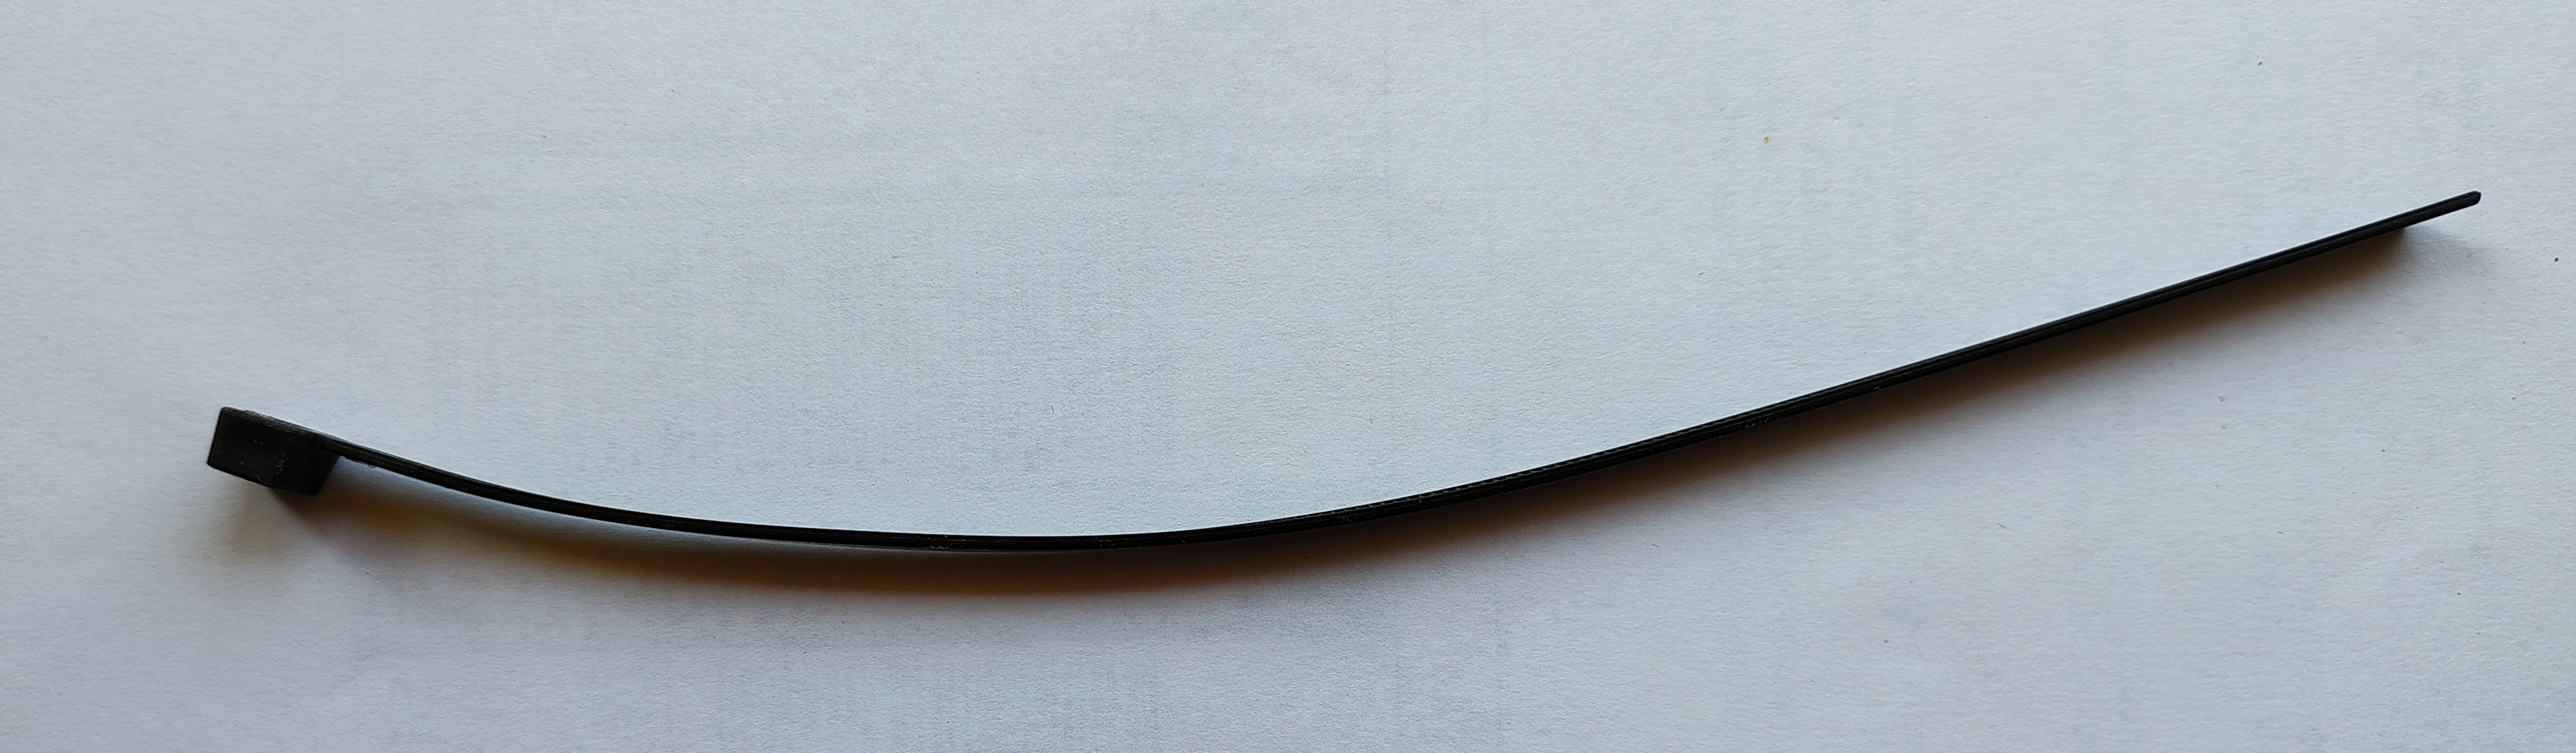
\includegraphics[width=0.8\textwidth]{figures/cable_tie.jpg}
    \caption{Kabelbinder}\label{fig:cable_tie}
    \end{figure}

\begin{figure}[H]
    \centering
    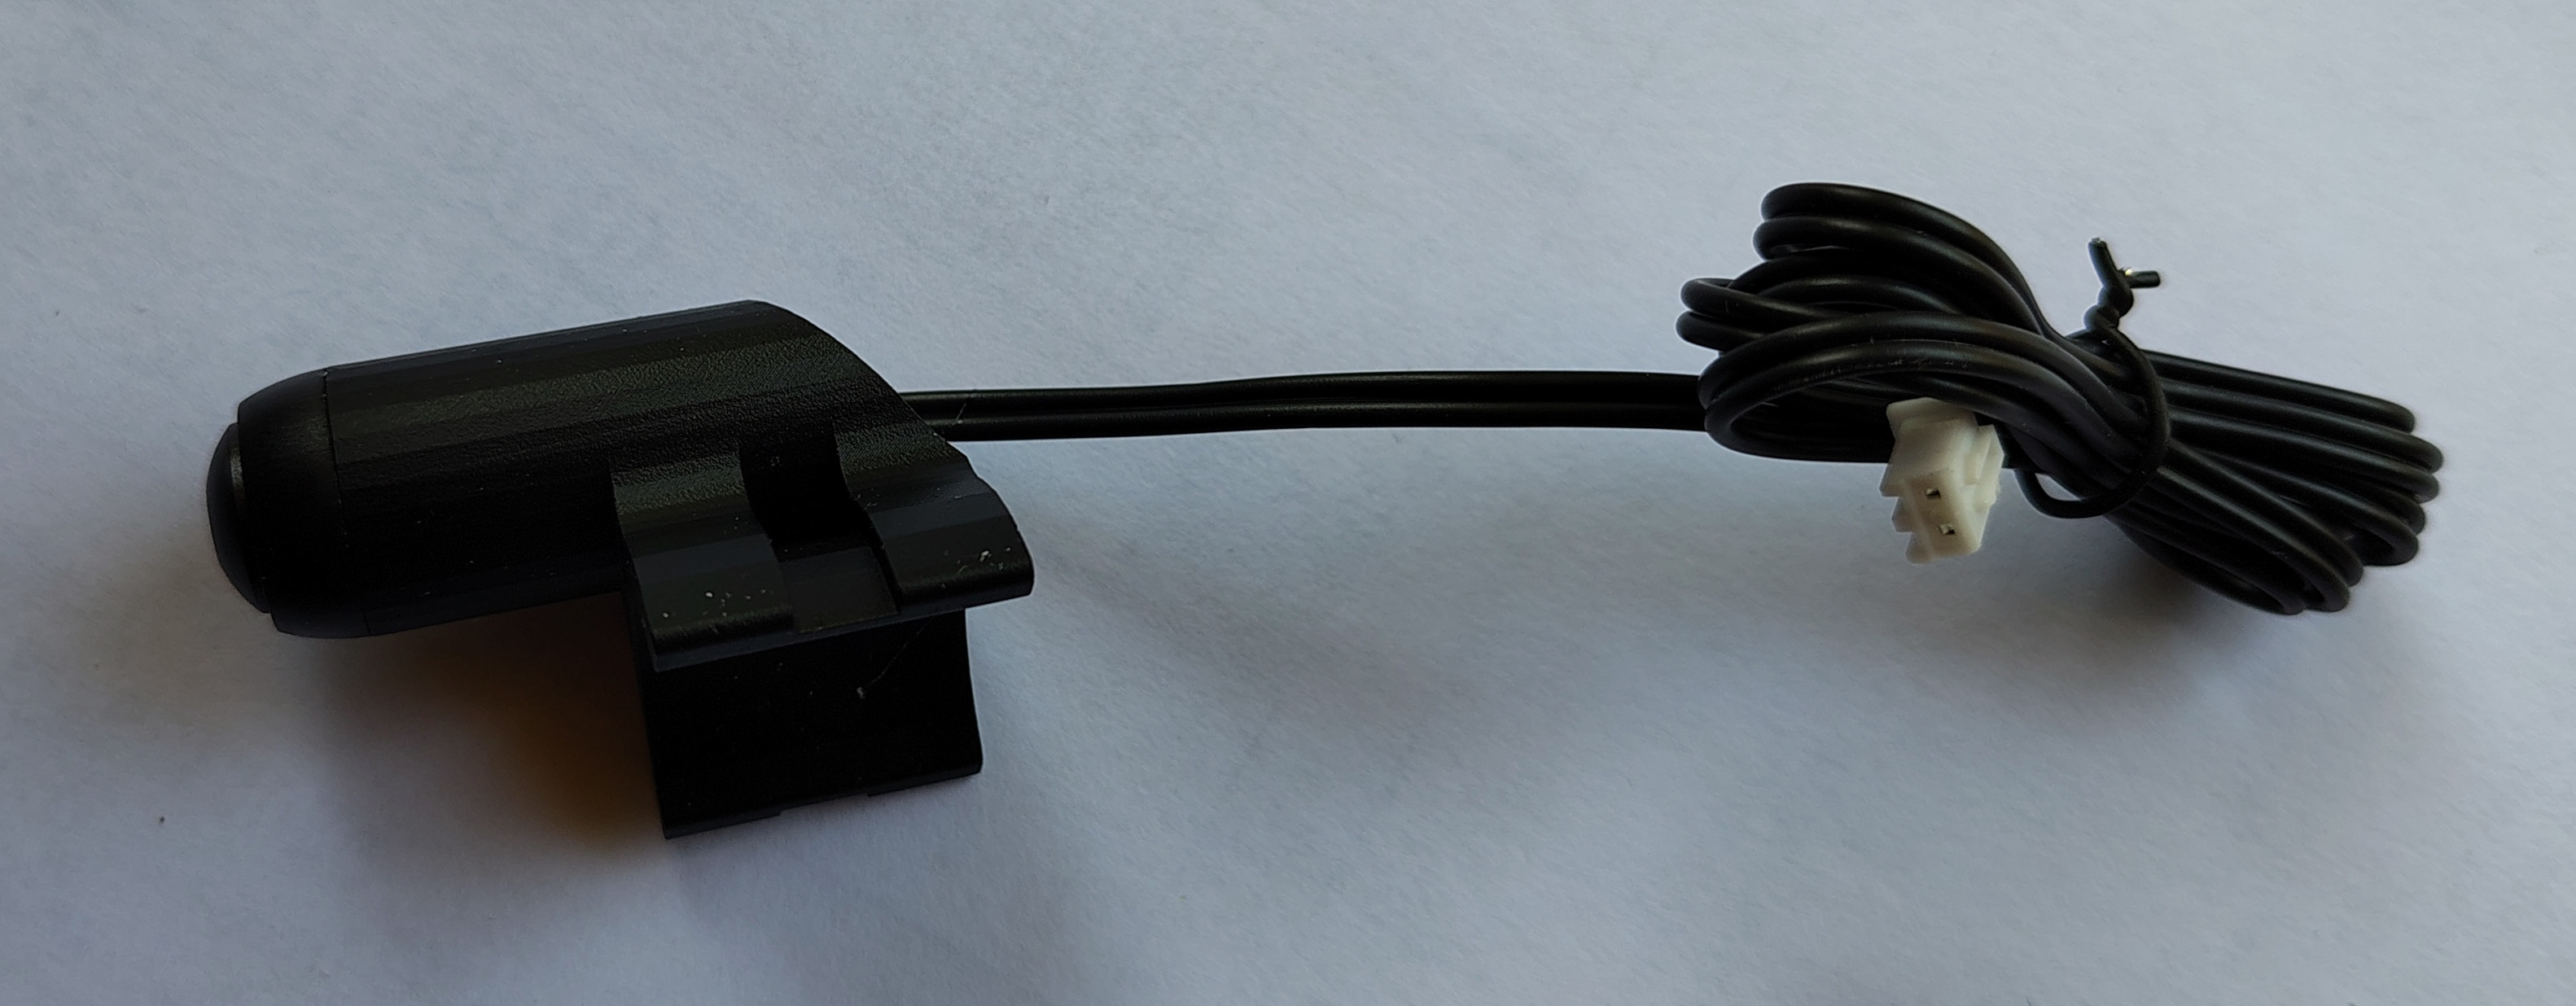
\includegraphics[width=0.8\textwidth]{figures/wiper_stalk_button.jpg}
    \caption{3D-gedruckter Knopf für den Wischerhebel}\label{fig:wiper_stalk_button}
    \end{figure}

\begin{figure}[H]
    \centering
    
\includegraphics[width=0.8\textwidth]{figures/sticker.png}
    \caption{ToM-Aufkleber}
\end{figure}